%%%%%%%%%%%%%%%%%%%%%%%%%%%%%%%%%%%%%%%%%%%%%%%%%
%%%              Document Class               %%%
%%%%%%%%%%%%%%%%%%%%%%%%%%%%%%%%%%%%%%%%%%%%%%%%%

\documentclass[12pt, a4paper, oneside]{report}
% remove comment, below, to compile only the specified chapter (for draft chapter compilations)
%%%%%%%%%%%%%%%%%%%%%%%%%%%%%%%%%%%%%%%%%%%%%%%%%
%%%   Basic Packages and Package Settings     %%%
%%%%%%%%%%%%%%%%%%%%%%%%%%%%%%%%%%%%%%%%%%%%%%%%%
%\usepackage{savesym}
\usepackage{multirow}
\usepackage{amssymb}
%\savesymbol{singleletter}								% American Mathematical Society symbols
\usepackage{float}												% customised float support
%\restoresymbol{X}{singleletter}
\usepackage{fancyhdr}											% improved header and footer support

\usepackage{amsmath}											% American Mathematical Society environments

\usepackage{makeidx}											% automatic index generation

\usepackage{url}												% URL typesetting
\usepackage{texnames}											% BIBTeX, SliTeX, AMSTeX, PiCTeX and TeXsis logos
\usepackage{verbatim}											% multi-line comments
\usepackage{ifpdf}												% selective setup for PDF compilation
\usepackage[number=none]{glossary}		
\usepackage{algorithmicx}

\usepackage{algcompatible}
\usepackage{algorithm}% http://ctan.org/pkg/algorithms
\usepackage{algpseudocode}% http://ctan.org/pkg/algorithmicx
\usepackage{breqn}
\usepackage{tikz}
\usepackage[%
    style=numeric-comp,sorting=none,
    sortcites=true,doi=false,url=false,
    giveninits=true,hyperref,backend=bibtex]{biblatex}

\usetikzlibrary{shapes.geometric, arrows, decorations.text, fit}
				% glossary file environments
\tikzstyle{process} = [rectangle, minimum width=3cm, minimum height=1cm, text centered, draw=black]
\tikzstyle{arrow} = [thick,->,>=stealth]
\tikzstyle{initial}=[circle,draw=black,text=black,text centered,minimum width=1cm,minimum height=1cm]


%%%%%%%%%%%%%%%%%%%%%%%%%%%%%%%%%%%%%%%%%%%%%%%%%
%%%          PDFLaTeX-Specific setup          %%%
%%%%%%%%%%%%%%%%%%%%%%%%%%%%%%%%%%%%%%%%%%%%%%%%%

\ifpdf

% PDFLaTeX-specific packages

\usepackage[
	pdftex,															% hyperlinked references for PDF output
	bookmarks=true,												% (option) build bookmarks
	bookmarksnumbered=true										% (option) add section numbers to bookmarks
]{hyperref}

\usepackage{pdfpages}											% required for PDF watermarking
\usepackage{epstopdf}											% automatic conversion of EPS images
\usepackage[pdftex]{thumbpdf}									% thumbnail generation for PDF files
\usepackage{pdflscape}											% required by thumbpdf
\usepackage[all]{hypcap}										% correct PDF figure links to top of image

% setup options for hyperlinks

\hypersetup{
	pdfhighlight=/N,												% (option) no visual cue on clicking link
	pdffitwindow=true,											% (option)
	pdfstartview=Fit,												% (option) fit initial view to page
	plainpages=false,												% (option) prevent hyperref page number changes
	breaklinks=true,												% (option) allow link breaking across lines
	colorlinks=true,												% (option) color link text only (no borders)
	pageanchor=false,												% (option) turns off page referencing for title page
	linkcolor=blue,												% (option) internal link color
	citecolor=blue,												% (option) citation link color
	filecolor=blue,												% (option) file link color
	menucolor=blue,												% (option) Acrobat menu link color
	pagecolor=blue,												% (option) page link color
	urlcolor=blue,													% (option) URL link color
}

% PDF meta-data settings

\hypersetup{
	pdftitle    = {A Very Long PhD Thesis With a Long Title},
	pdfauthor   = {Joseph Thomas Bloggs <jtbloggs@somewhere.co.za>},
	pdfsubject  = {Some sort of subject (e.g. Data mining)},
	pdfkeywords = {First keyword, second keyword, third keyword},
}

% force LaTeX-compliant spacing

\pdfadjustspacing=1

%%%%%%%%%%%%%%%%%%%%%%%%%%%%%%%%%%%%%%%%%%%%%%%%%
%%%       DVI/PostScript-Specific setup       %%%
%%%%%%%%%%%%%%%%%%%%%%%%%%%%%%%%%%%%%%%%%%%%%%%%%

\else

\usepackage{graphicx}											% EPS graphics

\fi

\usepackage{epstopdf}
\usepackage{caption}
\usepackage{subcaption}
\usepackage{csvsimple}
\usepackage{booktabs} 
\usepackage{pifont}
\newcommand{\cmark}{\ding{51}}
\newcommand{\xmark}{\ding{55}}

%%%%%%%%%%%%%%%%%%%%%%%%%%%%%%%%%%%%%%%%%%%%%%%%%
%%%                  Lengths                  %%%
%%%%%%%%%%%%%%%%%%%%%%%%%%%%%%%%%%%%%%%%%%%%%%%%%

\setlength{\textwidth}{158mm}
\setlength{\hoffset}{4.5mm}
\setlength{\headheight}{15pt}
\setlength{\unitlength}{1pt}
\setlength{\footnotesep}{5mm}

\ifpdf
	% ensure PDF is centered in display
	\setlength{\hoffset}{-10.5mm}
\else
	% add gutter margin for DVI/PostScript
	\setlength{\hoffset}{-10.5mm}
	\addtolength{\hoffset}{4.5mm}
\fi

%%%%%%%%%%%%%%%%%%%%%%%%%%%%%%%%%%%%%%%%%%%%%%%%%
%%%               Line Spacing                %%%
%%%%%%%%%%%%%%%%%%%%%%%%%%%%%%%%%%%%%%%%%%%%%%%%%

\newlength{\originalbaselineskip}
\setlength{\originalbaselineskip}{\baselineskip}
\linespread{1.3}

%%%%%%%%%%%%%%%%%%%%%%%%%%%%%%%%%%%%%%%%%%%%%%%%%
%%%               List Counters               %%%
%%%%%%%%%%%%%%%%%%%%%%%%%%%%%%%%%%%%%%%%%%%%%%%%%



%%%%%%%%%%%%%%%%%%%%%%%%%%%%%%%%%%%%%%%%%%%%%%%%%
%%%         Index and Glossary Terms          %%%
%%%%%%%%%%%%%%%%%%%%%%%%%%%%%%%%%%%%%%%%%%%%%%%%%

\renewcommand{\glossaryname}{Acronyms}
\renewcommand{\gloskip}{}
\setlength{\namewidth}{60pt}

\ifpdf
	\newcommand{\idxbf}[1]{\textbf{\hyperpage{#1}}}
\else
	\newcommand{\idxbf}[1]{\textbf{#1}}
\fi

\makeglossary
\makeindex

%%%%%%%%%%%%%%%%%%%%%%%%%%%%%%%%%%%%%%%%%%%%%%%%%
%%%        Figures and Floating Bodies        %%%
%%%%%%%%%%%%%%%%%%%%%%%%%%%%%%%%%%%%%%%%%%%%%%%%%

\renewcommand{\topfraction}{0.9}
\renewcommand{\bottomfraction}{0.0}
\renewcommand{\textfraction}{0.1}
\renewcommand{\floatpagefraction}{0.9}
\setcounter{topnumber}{1}
\setcounter{bottomnumber}{0}
\newfloat{graph}{tbp}{lgf}[chapter]
\floatname{graph}{Graph}
\newfloat{algorithm}{tbp}{loa}[chapter]
\floatname{algorithm}{Algorithm}

% bold float caption numbers and reduced size captions
\makeatletter
\long\def\@makecaption#1#2{%
	\vskip\abovecaptionskip
	\sbox\@tempboxa{{\small{\bf #1:} #2}}%
	\ifdim \wd\@tempboxa >\hsize
		{\small{\bf #1:} #2\par}
	\else
		\hbox to\hsize{\hfil\box\@tempboxa\hfil}%
	\fi
	\vskip\belowcaptionskip
}
\renewcommand\floatc@plain[2]{
	\setbox\@tempboxa\hbox{\small{\bf #1:} #2}%
	\ifdim\wd\@tempboxa>\hsize
		{\small{\bf #1:} #2\par}
	\else
		\hbox to\hsize{\hfil\box\@tempboxa\hfil}\fi}
\makeatother

\newlength{\abovesubfiglabelskip}
\setlength{\abovesubfiglabelskip}{0.5\abovecaptionskip}


\addbibresource{thesis.bib}

\begin{document}
%%%%%%%%%%%%%%%%%%%%%%%%%%%%%%%%%%%%%%%%%%%%%%%%%
%%%             Glossary Acronyms             %%%
%%%%%%%%%%%%%%%%%%%%%%%%%%%%%%%%%%%%%%%%%%%%%%%%%

\newacronym{AI}{Artificial Intelligence}{name=AI, description=Artificial Intelligence}
\newacronym{ANN}{Artificial Neural Network}{name=ANN, description=Artificial Neural Network}
\newacronym{CI}{Computational Intelligence}{name=CI, description=Computational Intelligence}

% and any other acronyms you want to use...

%%%%%%%%%%%%%%%%%%%%%%%%%%%%%%%%%%%%%%%%%%%%%%%%%
%%%           Index Sub-References            %%%
%%%%%%%%%%%%%%%%%%%%%%%%%%%%%%%%%%%%%%%%%%%%%%%%%

\index{AI|see{Artificial Intelligence}}
\index{ANN|see{Artificial Neural Network}}
\index{CI|see{Computational Intelligence}}

%%%%%%%%%%%%%%%%%%%%%%%%%%%%%%%%%%%%%%%%%%%%%%%%%
%%%%%%%%%%%%%%%%%%%%%%%%%%%%%%%%%%%%%%%%%%%%%%%%%

%%%%%%%%%%%%%%%%%%%%%%%%%%%%%%%%%%%%%%%%%%%%%%%%%
%%%%%%%%%%%%%%%%%%%%%%%%%%%%%%%%%%%%%%%%%%%%%%%%%

\newlength{\negativetitlepageoffset}
\setlength{\negativetitlepageoffset}{-5cm}

\begin{titlepage}
	\ \vspace{\negativetitlepageoffset}
	\vspace{\stretch{1}}
	\setlength{\baselineskip}{2.4\originalbaselineskip}
	\begin{center}
		\textsf{\huge Nature-based Algorithms for Prioritized Foraging}
	\end{center}
	\begin{center}
		\textsf{by}
	\end{center}
	\begin{center}
		\textsf{\large Jade Zoe Abbott}
	\end{center}
	\vspace{\stretch{1}}
	\setlength{\baselineskip}{1.3\originalbaselineskip}
	\begin{center}
		\textsf{Submitted in partial fulfillment of the requirements for the degree\\
		Master of Science (Computer Science)\\
		in the Faculty of Engineering, Built Environment and Information Technology\\
		University of Pretoria, Pretoria}
	\end{center}
	\vspace{0.15cm}
	\centerline{
		\textsf{December 2013}
	}
\end{titlepage}

%%%%%%%%%%%%%%%%%%%%%%%%%%%%%%%%%%%%%%%%%%%%%%%%%
%%%%%%%%%%%%%%%%%%%%%%%%%%%%%%%%%%%%%%%%%%%%%%%%%

\pagestyle{empty}
\newpage

\textsf{\small
	\vfill
	\noindent Publication data:\\*[2.5mm]
	\parbox{\textwidth}{
		\fontsize{9}{10pt}
		\selectfont
		Jade Zoe Abbott. Nature-based Algorithms for Prioritized Foraging. Masters thesis, University of Pretoria, Department of Computer Science, Pretoria, South Africa ,December 2013.
	}\\*[10.5mm]
	Electronic, hyperlinked versions of this thesis are available online, as Adobe PDF files, at:\\*[2.5mm]
	\parbox{\textwidth}{
		\fontsize{9}{9.5pt}
		\selectfont
		\url{http://cirg.cs.up.ac.za/}\\*[1.5mm]
		\url{http://upetd.up.ac.za/UPeTD.htm}
	}
}

%%%%%%%%%%%%%%%%%%%%%%%%%%%%%%%%%%%%%%%%%%%%%%%%%
%%%%%%%%%%%%%%%%%%%%%%%%%%%%%%%%%%%%%%%%%%%%%%%%%

\newpage

\begin{center}
	{\large\bf Nature-based Algorithms for Prioritized Foraging}
\end{center}
\begin{center}by\end{center}
\begin{center}
	{Jade Zoe Abbott}\\
	\ifpdf
		E-mail: \href{mailto:jabbott@cs.up.ac.za}{jabbott@cs.up.ac.za}
	\else
		E-mail: jabbott@cs.up.ac.za
	\fi
\end{center}
\vspace{1cm}
\begin{center}{\large\bf Abstract}\end{center}
Your thesis abstract goes here. This should be a single paragraph. Try to keep it as brief as possible (less than 200 words --- if this abstract page runs onto a second page, it needs shortening), while keeping in mind that it should touch on all the important aspects of your research --- consider whether someone unfamiliar with your research area would be able to determine whether your research is relevant to them, or not. Keep in mind that the abstract may be the only thing someone reads before choosing to either discard your work, or keep reading. Also, make sure that there are no references in the abstract. The keywords list should include no more than ten keywords. Keywords may be single words, or multi-word terms (such as ``neural networks'' or ``particle swarm optimisers''). When choosing keywords, consider terms that are descriptive of your research, and are likely to be used in search queries that should find your work.

\noindent\

\noindent{\bf Keywords:} First keyword, second keyword, final keyword.

\vfill
\noindent
{\bf\parbox{26.8mm}{Supervisors}:} Prof.~S. U. P. Visor \\* % only provide titles of Prof. or Dr. (not Mr.)
{\bf\parbox{28.55mm}{~}} Dr.~A. N. Other \\*
%{\bf\parbox{26.8mm}{Supervisor}:} Prof.~S. U. P. Visor \\* % if you only have a single supervisor
{\bf\parbox{26.8mm}{Department}:} Department of Computer Science \\*
{\bf\parbox{26.8mm}{Degree}:} Master of Science

%%%%%%%%%%%%%%%%%%%%%%%%%%%%%%%%%%%%%%%%%%%%%%%%%
%%%%%%%%%%%%%%%%%%%%%%%%%%%%%%%%%%%%%%%%%%%%%%%%%

\newpage

\ \vspace{\stretch{1}}

\begin{quotation}
``The Three Laws of Robotics:

1: A robot may not injure a human being or, through inaction, allow a human being to come to harm;

2: A robot must obey the orders given it by human beings except where such orders would conflict with the First Law;

3: A robot must protect its own existence as long as such protection does not conflict with the First or Second Law;''
\end{quotation}
\begin{flushright}
Isaac Asimov, I, Robot
\end{flushright}

\vspace{1cm}

\begin{quotation}
``Another quote, if you feel like it\ldots''
\end{quotation}
\begin{flushright}
Another Quote attribution or source (1890)
\end{flushright}

\ \vspace{\stretch{1}}

%%%%%%%%%%%%%%%%%%%%%%%%%%%%%%%%%%%%%%%%%%%%%%%%%
%%%%%%%%%%%%%%%%%%%%%%%%%%%%%%%%%%%%%%%%%%%%%%%%%

\newpage

\begin{center}{\Large\bf Acknowledgements}\end{center}

\vspace{0.3cm}

\noindent If you wish to include any acknowledgements to anyone you feel was instrumental in the completion of the thesis (or your continued survival through it's completion):
\begin{itemize}
	\item First person (or institution) you'd like to thank, and reasons;

	\item Second person (or institution), and reasons;

	\item Final person (or institution), and reasons.
\end{itemize}

%%%%%%%%%%%%%%%%%%%%%%%%%%%%%%%%%%%%%%%%%%%%%%%%%
%%%%%%%%%%%%%%%%%%%%%%%%%%%%%%%%%%%%%%%%%%%%%%%%%

\cleardoublepage
\pagestyle{plain}
\pagenumbering{roman}
\setcounter{page}{1}
\ifpdf
\pdfbookmark[0]{Contents}{contents}
\fi
\tableofcontents

%%%%%%%%%%%%%%%%%%%%%%%%%%%%%%%%%%%%%%%%%%%%%%%%%
%%%%%%%%%%%%%%%%%%%%%%%%%%%%%%%%%%%%%%%%%%%%%%%%%

\cleardoublepage
\ifpdf
\phantomsection
\fi
\addcontentsline{toc}{chapter}{List of Figures}
\listoffigures

%%%%%%%%%%%%%%%%%%%%%%%%%%%%%%%%%%%%%%%%%%%%%%%%%
%%%%%%%%%%%%%%%%%%%%%%%%%%%%%%%%%%%%%%%%%%%%%%%%%

\cleardoublepage
\ifpdf
\phantomsection
\fi
\addcontentsline{toc}{chapter}{List of Graphs}
\listof{graph}{List of Graphs}

%%%%%%%%%%%%%%%%%%%%%%%%%%%%%%%%%%%%%%%%%%%%%%%%%
%%%%%%%%%%%%%%%%%%%%%%%%%%%%%%%%%%%%%%%%%%%%%%%%%

\cleardoublepage
\ifpdf
\phantomsection
\fi
\addcontentsline{toc}{chapter}{List of Algorithms}
\listof{algorithm}{List of Algorithms}

%%%%%%%%%%%%%%%%%%%%%%%%%%%%%%%%%%%%%%%%%%%%%%%%%
%%%%%%%%%%%%%%%%%%%%%%%%%%%%%%%%%%%%%%%%%%%%%%%%%

\cleardoublepage
\ifpdf
\phantomsection
\fi
\addcontentsline{toc}{chapter}{List of Tables}
\listoftables

%%%%%%%%%%%%%%%%%%%%%%%%%%%%%%%%%%%%%%%%%%%%%%%%%
%%%%%%%%%%%%%%%%%%%%%%%%%%%%%%%%%%%%%%%%%%%%%%%%%

%%%%%%%%%%%%%%%%%%%%%%%%%%%%%%%%%%%%%%%%%%%%%%%%%
%%%%%%%%%%%%%%%%%%%%%%%%%%%%%%%%%%%%%%%%%%%%%%%%%

\ifpdf
\hypersetup{pageanchor=true}									% (option) turn page referencing back on for chapters
\fi

\pagestyle{fancy}
\fancypagestyle{headings}{
	\fancyhead[RO,LE]{\thepage}
	\fancyhead[LO]{\sf\nouppercase{\leftmark}}
	\fancyhead[RE]{\sf\nouppercase{\rightmark}}
	\fancyfoot{}
	\renewcommand{\headrulewidth}{0.4pt}
}


%%%%%%%%%%%%%%%%%%%%%%%%%%%%%%%%%%%%%%%%%%%%%%%%%
%%%%%%%%%%%%%%%%%%%%%%%%%%%%%%%%%%%%%%%%%%%%%%%%%

\chapter{Introduction}
\label{chap:introduction}
\pagestyle{headings}
\pagenumbering{arabic}
\setcounter{page}{1}

%%%%%%%%%%%%%%%%%%%%%%%%%%%%%%%%%%%%%%%%%%%%%%%%%
%%%%%%%%%%%%%%%%%%%%%%%%%%%%%%%%%%%%%%%%%%%%%%%%%

Section~\ref{sec:introduction:motivation} motivates the purpose of this thesis, and the objectives of this thesis are highlighted in Section~\ref{sec:introduction:objectives}. The contributions of the thesis are presented in Section~\ref{sec:introduction:contributions}, while Section~\ref{sec:introduction:outline} outlines the the structure of the thesis.
%%%%%%%%%%%%%%%%%%%%%%%%%%%%%%%%%%%%%%%%%%%%%%%%%
%%%%%%%%%%%%%%%%%%%%%%%%%%%%%%%%%%%%%%%%%%%%%%%%%

\section{Motivation}
\label{sec:introduction:motivation}
Consider a search and rescue mission after a natural disaster or mining accident. These search and rescue missions are usually extremely dangerous for the human rescuers who are deployed to search for survivors. The use of swarm robotics to perform such search and rescue mission has been proposed and explored as an alternative to using human rescuers \cite{murphy2008search,naghsh2008analysis}.

Swarm robotics is the co-coordination of large numbers of  relatively simple robots to perform a single collaborative function. Swarm robotics is inspired from the observation of social insects such as ants, termites, and bees \cite{dorigo2004swarm}. An important activity of all natural swarms is foraging for resources. Foraging is defined as the search and collection of resources from sources in an environment and returning the resources to a collection point \cite{winfield2009foraging}. These resources could be food, water, or building materials. Foraging is an abstraction of the search and rescue problem where the trapped humans are items that robots need to locate and remove to a safe location. 

In a search and rescue mission, the location of trapped humans is usually unknown and humans can be potentially be blocked by rubble, which needs to be removed before the humans can be safely removed. A swarm of robots would need to search for the humans, as fast as possible, to avoid further danger, injury or loss of life. If robots cannot locate the humans, they will have to begin clearing debris in the hope of locating them, as well as clearing the route between the trapped humans and the safe zone. Locating and removing the humans is prioritized above removal of the debris, but often the debris must be removed, in order to locate the trapped humans. Thus there exists a resource prioritization from the perspective of the robot.

Resource prioritization is also relevant in mining problems where the metal ore is prioritized and the waste rock should be cleared to better access the valuable ore. In common gold mining techniques, the ore and waste rock are collected and transported to the surface and chemical techniques are used to separate them. The transport of the waste rock (which forms the majority of the load) to the surface is extremely expensive, so there is a cost benefit to separate the ore and the waste rock beneath the surface and transport only the valuable ore to the surface.

The above search and rescue problem and mining problem can be abstracted as a foraging problem where there exists resources with differing priorities. In the case of search and rescue, the humans are the prioritized resource and the debris is the non-prioritized resource. In mining, the ore is the prioritized resource and the waste rock is the non-prioritized resource. 

In nature, in times of stress, the collection of one resource may be prioritized over others - such as water during a drought or food before winter. Individuals in a natural swarm often adapt behaviour appropriately to enable greater collection of the prioritized item.

This study defines the prioritized foraging problem, and proposes three swarm robotics foraging algorithms to be evaluated on the prioritized foraging problem. The study proposes metrics to evaluate each algorithm's performance on the prioritized foraging problem in terms of foraging efficiency, flexibility, scalability and robustness. The algorithms are developed in a simulated environment. Each algorithm's performance is evaluated on environments of a variety of complexities, with various swarm configurations.

%%%%%%%%%%%%%%%%%%%%%%%%%%%%%%%%%%%%%%%%%%%%%%%%%
%%%%%%%%%%%%%%%%%%%%%%%%%%%%%%%%%%%%%%%%%%%%%%%%%

\section{Objectives}
\label{sec:introduction:objectives}

The primary objectives of this thesis are as follows: To

\begin{itemize}
	\item conduct a survey of the swarm robotics field;
	\item conduct a survey of foraging in social insects and  swarm robotics;
	\item define the prioritized foraging problem;
	\item propose metrics for evaluating the performance of swarm robotics algorithms on the prioritized foraging problem;
	\item propose and develop different nature-inspired algorithms in a simulated swarm robotic environment, to be evaluated on the prioritized foraging problem; and
	\item evaluate the efficiency, flexibility, scalability, and robustness of the nature-inspired algorithms over different environments and different swarm configurations on the prioritized foraging problem.
\end{itemize}


%%%%%%%%%%%%%%%%%%%%%%%%%%%%%%%%%%%%%%%%%%%%%%%%%
%%%%%%%%%%%%%%%%%%%%%%%%%%%%%%%%%%%%%%%%%%%%%%%%%

\section{Contributions}
\label{sec:introduction:contributions}

The thesis makes the following contributions:

\begin{itemize}
	\item A novel variation of the foraging problem, i.e. prioritized foraging, as well as performance measures for the prioritized foraging problem are proposed.
	\item A novel honey bee inspired foraging algorithm for robot swarms is developed.
	\item A novel obstacle avoidance algorithm, inspired by the flocking behaviour of birds is developed.
	\item Methods for generating various types of foraging environments in a simulated environments are proposed.
	\item An analysis of the efficiency, flexibility, scalability, and robustness of each algorithm on the prioritized foraging problem is conducted.
\end{itemize}


%%%%%%%%%%%%%%%%%%%%%%%%%%%%%%%%%%%%%%%%%%%%%%%%%
%%%%%%%%%%%%%%%%%%%%%%%%%%%%%%%%%%%%%%%%%%%%%%%%%

\section{Thesis Outline}
\label{sec:introduction:outline}
This thesis consists of eight chapters, each handling a separate topic. The chapters are as follows:

\begin{itemize}
\item\textbf{Chapter~\ref{chap:first}} introduces the origin, motivation, development and current state of swarm robotics.

\item\textbf{Chapter~\ref{chap:second}} summarizes foraging behaviour of social insects and reviews existing foraging algorithms in swarm robotics.

\item\textbf{Chapter~\ref{chap:divisionoflabour}} defines division of labour and summarizes strategies for division of labour employed by social insects. The chapter reviews where division of labour strategies have been employed by robot swarms.

\item\textbf{Chapter~\ref{chap:third}} proposes a novel foraging variation called prioritized foraging. The chapter also proposes three swarm robotic foraging algorithms, inspired by social insects, to be evaluated on a prioritized foraging problem.

\item\textbf{Chapter~\ref{chap:experiment}} presents an experiment designed to evaluate the proposed foraging algorithms in a simplified simulation environment, on the prioritized foraging problem. This chapter describes the environment and swarm parameters that the experiments use. The relevant performance measures to be used to evaluate the proposed algorithms on the prioritized foraging problem are also presented.

\item\textbf{Chapter~\ref{chap:results}} analyses the results of applying the proposed algorithms to the prioritized foraging problem.

\item\textbf{Chapter~\ref{chap:conclusions}} summarizes the findings of this research.

\end{itemize}

The thesis contains two appendices, which are organised as follows:

\begin{itemize}
\item\textbf{Appendix~\ref{app:acronyms}} provides a list of important acronyms that are used in the course of this work, along with their definitions

\item\textbf{Appendix~\ref{app:symbols}} lists and defines the mathematical symbols used in this thesis, divided according to the chapter in which they appear.

%\item\textbf{Appendix~\ref{app:derived_publications}} contains the publications derived from this work.

\end{itemize}




%You might also include a page reference to the index (if you decide to include one) here, as follows: page~\pageref{index}.

%Please refer to the bibliography database (in the file \texttt{bibliography.bib}) for a skeleton of how you would add references to your work. You cite them in your text, in any order you need, as follows: \cite{ref:Alhoniemi:1999b}, \cite{ref:Alahakoon:2000}, \cite{ref:Oja:2003}, \cite{ref:Alhoniemi:1999a}, \cite{ref:Kaski:1995}, \cite{ref:Fasulo:1999}, \cite{ref:Kaski:1997} and \cite{ref:Aha:1998}. You may include extra page information as follows: \cite{ref:Clark:1989}[page~82]. Note that references will only show up in the bibliography once you actually cite them in the document. The entries will also be alphabetised automatically.

%Make sure that the bibliographic information is as accurate as possible. Provide full author names, as they appear on the paper. Make sure you provide as much information as possible, but try to keep it relatively brief as well (for example, include minimal information in the address field). Make absolutely sure that references are correct, since there are a large number of incorrect ones listed in published articles.

%Note that references to online resources should only be provided in instances when a document's primary publication method is online. You may also provide a reference to a Digital Object Identifier (DOI)\footnote{A DOI is a unique alphanumeric identification string for a digital object, providing a persistent link to it. It represents a permanent URL kept the same way a domain name is. For further information on DOI, see \url{http://www.doi.org}. Publication DOIs are provided in the CrossRef framework. CrossRef is a non-profit network providing infrastructure for linking online citations, using the DOIs of documents that are available electronically. CrossRef DOIs looks something like \texttt{doi:10.1234/5678}, and work like standard hyperlinks in most web browsers (you can past them into the address bar of a browser and you will be taken directly to the online document). DOIs may also be manually resolved via \url{http://dx.doi.org}. For more information on CrossRef, see \url{http://www.crossref.org}.} if one is available, but this should always be provided in conjunction with the physical publication details (note that many journals and conferences will still have a problem with DOIs being cited, since they are online documents, even though they are persistent).

%After you have discussed the chapters, provide a brief introduction for the list of appendices:
%\begin{itemize}
%	\item\textbf{Appendix~\ref{app:appendix1}} describes \ldots.
	
%	\item\textbf{Appendix~\ref{app:appendix2}} covers \ldots.
	
%	\item\textbf{Appendix~\ref{app:acronyms}} provides a list of the important acronyms used or newly defined in the course of this work, as well as their associated definitions.
	
%	\item\textbf{Appendix~\ref{app:symbols}} lists and defines the mathematical symbols used in this work, categorised according to the relevant chapter in which they appear.
	
%	\item\textbf{Appendix~\ref{app:derived_publications}} lists the publications derived from this work.
%\end{itemize}

%If you provide an index, you may provide a page reference here, indicating that it begins on page~\pageref{index} of the text.

%%%%%%%%%%%%%%%%%%%%%%%%%%%%%%%%%%%%%%%%%%%%%%%%%
%%%%%%%%%%%%%%%%%%%%%%%%%%%%%%%%%%%%%%%%%%%%%%%%%
%%%%%%%%%%%%%%%%%%%%%%%%%%%%%%%%%%%%%%%%%%%%%%%%%
%%%%%%%%%%%%%%%%%%%%%%%%%%%%%%%%%%%%%%%%%%%%%%%%%

\chapter{Swarm Robotics}
\label{chap:first}

%%%%%%%%%%%%%%%%%%%%%%%%%%%%%%%%%%%%%%%%%%%%%%%%%
%%%%%%%%%%%%%%%%%%%%%%%%%%%%%%%%%%%%%%%%%%%%%%%%%

This chapter provides a broad view of swarm robotics in terms of its origin, motivation, development and current state.
Section~\ref{sec:first:definitionswarmrobotics} defines the concept of swarm robotics while the origin and a brief history of swarm robotics is provided in Section~\ref{history}. Motivations for swarm robotics are outlined in Section~\ref{motivations}, followed by Section~\ref{currentstate} which expands on the current state of swarm robotics. Lastly, the chapter addresses the challenges faced by swarm robotics in Section~\ref{challenges}.

%%%%%%%%%%%%%%%%%%%%%%%%%%%%%%%%%%%%%%%%%%%%%%%%%
%%%%%%%%%%%%%%%%%%%%%%%%%%%%%%%%%%%%%%%%%%%%%%%%%

\section{What is Swarm Robotics?}
\label{sec:first:definitionswarmrobotics}

Swarm robotics is the study of the co-coordination of large numbers of relatively simple robots in order to perform a single function, without the existence of central control. Swarm robotics focuses on how to create robotic algorithms that result in the emergence of a desired complex behaviour \cite{csahin2005swarm}.

Swarm robotics typically draws inspiration from the observation of social insects, for example, ants \cite{hoff2010two}, cockroaches \cite{garnier2005aggregation} and bees \cite{lee2012foraging} who exhibit collective behaviour in the growth and maintenance of their societies \cite{wilson1971insect}. Social insect societies exhibit desired qualities of a robot swarm, namely robustness, scalability and flexibility. Swarm robotics also draws on concepts from other societies such as the amoeba's aggregation into slime \cite{schmickl2007navigation} and communication, propulsion and sensing in bacteria \cite{dhariwal2004bacterium,martel2010using}. 

\section{Motivations for Swarm Robotics}
\label{motivations}

Swarm robots draws inspiration from insect swarms due to the characteristics of robustness, flexibility, scalability and to a lesser extent cost-effectiveness. The following sections describe the characteristics of insect swarms that all swarm robotics algorithms strive to achieve. 

\subsection{Robustness}
\label{robustness}


In swarm robotics, robustness is defined as the ability of a swarm to continue to perform it's function, despite failures or abnormalities of the respective individuals and environments. Three aspects of insect swarm algorithms have been identified as enabling robustness: redundancy, decentralized coordination, and multiplicity of sensing \cite{csahin2005swarm}.

Swarm robotics algorithms achieve redundancy by giving all, or a portion of the robots in the swarm the same capabilities. In this way, if a percentage of the swarm malfunctions, the other robots have the capability to take the malfunctioning robots' place. The loss of a single individual is compensated by another individual in the swarm.

Decentralized coordination can be attained by creating algorithms that do not depend on the life span of any single individual or a few individuals of the swarm.

The use of a large number of individuals increases the total number of sensors in the swarm. As a result of the sensory multiplicity, the total signal-to-noise ratio is increased. If the sensor data of the robot swarm is adequately aggregated by the swarm, the overall effect of noise can be decreased or eliminated. 

\subsection{Flexibility}
\label{flexibility}

A swarm robotics algorithm should exhibit the ability to adapt and adjust to a wide variety of different environments and tasks \cite{brambilla2013swarm}. Ants and bees do this by having effective division of labour strategies. The individuals in many insect societies can take on a variety of different roles required by the nest such as brooding, foraging or nest maintenance, due to changes in the environment \cite{morley1946division}. The ability to take on different roles when requirements change, is known as division of labour \cite{beshers2001models}. Many swarm robotics algorithms make use of the division of labour strategies of social insects, in order to adapt to changing requirements  \cite{gerkey2004formal, labella2006division, liu2007towards}. The use of division of labour thus assists the swarm in maintaining flexibility.

\subsection{Scalability}
\label{sr:scalabilty}
Scalability refers to the ability of the robotic swarm to expand the self-organizational mechanism, by simply adding more robots to the swarm \cite{brambilla2013swarm}. The performance of the algorithm should not be negatively effected by an increase in swarm size, and an increase in swarm size should adequately improve the performance of the swarm. Scalability studies should be performed in order to determine whether an algorithm's performance will increase or decrease at an adequate rate as the swarm size increases. Scalability studies have been performed in \cite{bahgecci2005evolving,nouyan2008path,zarzhitsky2005distributed}
Scalability consists of two dimensions: in terms of the scalability of the size of the swarm or in terms the size of the problem being solved \cite{brambilla2013swarm}.

\subsection{Cost-effectiveness}
The idea that swarm robotics is more cost effective than traditional robotics runs off the premise that multiple inexpensive robots are likely to be cheaper to buy and maintain than a single, large, more complex robot. 

\section{Characteristics of Swarm Robotics}
\label{characteristics}

Drawing from inspiration from social insects, swarm robotics algorithms have a number of characteristics that distinguish them from other robotics algorithms. The characteristics are as follows:

\begin{enumerate}

\item \textbf{Quantity}: Studies are regularly focused with scalability as a potential characteristic of swarm robotics algorithms - even if real-robot experimentation is limited to only a few individuals. In order to test the scalability of an algorithm, models or simulations are often built for experimentation purposes. Erol Sahin proposes that 10 individuals are a reasonable lower bound for a group of robots to be considered a swarm \cite{csahin2005swarm}. A group of robots with less than 10 robots, is considered just that - a group of robots. 

\item \textbf{Homogeneity}: A group of robots that has ``too many" individuals with unique characteristics, is no longer considered a swarm, since it would likely violate the robustness requirements. Robustness would be violated since loosing a specific robot, that is the only individual of its kind capable of performing a specific function, would mean that the swarm no longer can perform that function and is therefore, no longer robust. It is of the author's opinion that heterogeneity can exist in robot swarm provided that the redundancy of each type of robot in the swarm is high enough, or if the failure of that specific robot can be compensated for, even if only to a lesser efficiency, by the remaining types of robots. The evaluation of the degree of homogeneity of a swarm of robots has been discussed and a potential measure of homogeneity is proposed in \cite{balch2000hierarchic}.

\item \textbf{Decentralization and Autonomy}: There should be no single point of failure in the group of robots and the robots must have complete self-control of their actuation and sensors, without central control. Decentralization and autonomy of the robots are key factors enabling the robustness of the system. If a particular process requires a single leader to make a decision, such a process should include the ability to detect situations when a leader is no longer present (due to malfunction or destruction) and then to re-elect a new leader without human intervention, otherwise the swarm can no longer continue it's function at the failure of a single individual.

\item \textbf{Localization}: Assume a group of robots that are dependant on global sensors and communication - for example, all inter-robot communications have to pass through a centralized server, or an overhead camera that all individuals of the swarm connect to and use for navigation. The problem with global sensing or communication is that the swarm has a single point of failure, thus violating decentralization. Thus, local sensory and communication abilities are required in order to uphold the decentralization requirement. If sensor are local to each robot, when a single robot's local communications fail, then the rest of the swarm can still communicate (albeit, in a deteriorated manner).

\item \textbf{Simplicity}: A single robot should be under-equipped to handle the task by itself, however, collaboration amongst a group of the same robots should assist the completion of the task. In the author's opinion, the level of simplicity of robots is a topic worth debating since ``simple" is a relative term and various complexities of robots have been used in swarms. For example, the kilobot project \cite{rubenstein2012kilobot} has built very low cost simple robots to enable testing of collective behaviours on very large swarms. The kilobots do not even have wheels for motion but simply have a three rigid legs with vibration motors for actuation. Sensors are limited in the form of a simple ambient light sensor and an infrared transmitter and receiver, and coloured LED lights for communication. 

On the other side of the spectrum, Melliner \textit{et al} \cite{kushleyev2013towards, mellinger2013cooperative} explore robotics algorithms for swarms of relatively advanced, expensive quadcoptors with a variety of top-class sensors such as magnetometers, accelerometers, gyros, barometer for altitude sensing and two Zigbee transceivers for communication.
\end{enumerate}

 The field of swarm robotics has been applied to a large variety of problems such as search and rescue \cite{mondada2002search}, item or garbage collection \cite{balch1995io}, autonomous inspection of machinery \cite{correll2007challenging}, and military formations for military application \cite{balch1998behavior}.


%%%%%%%%%%%%%%%%%%%%%%%%%%%%%%%%%%%%%%%%%%%%%%%%%
%%%%%%%%%%%%%%%%%%%%%%%%%%%%%%%%%%%%%%%%%%%%%%%%%

\section{History}
\label{history}
 
%TODO: Turn into an introduction. 
Swarm robotics is simply the latest buzzword for a concept that has been of interest since the 1980s. Swarm Robotics has gone by many other names in the past. Early swarm robotics research explored the use of robots as a tool with which to model and validate entomology research on social insects \cite{dorigo2014swarm, beni1993swarm, seeley2009wisdom}.

This section aims to briefly highlight the history of swarm robotics and it's progress by addressing behaviour based robotics, the origins of multi-robot systems, and other early research.

\subsection{Journey from Classic Robotics}
\label{journeyfromtraditionalAI}

The first step in the movement from symbol-based classical robotics to swarm robotics was the movement from complex symbolic systems towards more simpler architectures which began in the mid-to-late 1980s. In Rodney A. Brooks' iconic paper ``Elephants don't play chess" \cite{brooks1990elephants}, the movement from traditional artificial intelligence, towards what they brand ``nouvelle" artificial intelligence, is discussed. Brooks explains that traditional symbol-based classical artificial intelligence made certain assumptions about how intelligence worked and those assumptions actually impeded traditional artificial intelligence techniques. 

Brooks presents the physical grounding hypothesis which is the idea that intelligence is composed of individual modules that generate behaviour and the co-existence and co-operation of these modules allow for the emergence of complex behaviour. The physical grounding hypothesis states that the world is its own best model and thus in order to accurately make decisions about the real world, one should add sensing and actuating capabilities to artificial intelligence agents.

On the other hand, classical or symbolic artificial intelligence (most notably used by systems such as Prolog) makes use of the symbol system hypothesis that states that all intelligence operates using symbols. The implication that symbols represent all world entities fails since symbols may not be up to date with the environment or have the ability to represent unseen things. 

The physical grounding hypothesis lead to the development of behaviour-based robotics and more concretely the subsumption architecture \cite{brooks1986robust} by tightly connecting perception to action. A subsumption program organises finite state machines into layered incremental networks. 

Multiple systems were developed using the subsumption architecture with great success. Allen, a robot that has three layers of behaviours: i.e. obstacle avoidance layer, a random wandering layer, and a search for the furthest point layer. These 3 separate behaviours cause the robot to adequately explore an environment \cite{brooks1986robust}.

Herbert, the soda can collector robot, was a notable development. Herbert was required to complete the significantly more complex task of search for and picking up empty soda cans from people's desks \cite{connell1989colony}. To solve the problem, 15 individual behaviours were developed, with no communication between the behaviour generating modules. Other subsumption implementations include Toto \cite{mataric1990distributed}, Squirt \cite{flynn1989world} and Genghis \cite{brooks1989robot}.

The key feature that can be determined from the success of physically grounded systems is that interactions of simpler non-goal directed behaviour results in emergence of goal-directed behaviour. Ronald Arkin discusses the idea that behaviour-based robotics imposes a biologically bottom up approach with the need that intelligence must be reactive to the dynamic environment and that intelligence needs to generate robust results despite noisy complex real world environments \cite{arkin1990integrating}.

Behaviour-based robotics is the idea that complex robot behaviour can emerge from a combination of simple behaviours. It is of the author's opinion that behaviour-based robotics signifies the a change in focus of robotics research, from complex indviduals robots, to complex robots composed of simple behaviours (behaviour-based robotics), and finally to multi-robot systems consisting of simple robots composed of simple behaviours. Most work in swarm robotics began after the introduction of the behaviour-based robotics paradigm \cite{arai2002editorial}.

\subsection{Evolution of the term ``Swarm Robotics" and early research}
\label{early-research}
%TODO: Make flow
%How to rearrange? Potentially remove?

Early research involving collaboration of multiple agents was originally a way of verifying entomology research on social insects \cite{dorigo2014swarm, beni1993swarm, seeley2009wisdom}. Many researchers modelled and simulated aspects of the insect colonies that were being studied in order to learn more about their self-organizational mechanisms. 

Early work included modeling the excavation behaviour and tunnel creation of ants in order to simulate the rate of excavation \cite{sudd1975model}. Agent simulation was used to validate a model of the spatial arrangement and diet overlap between colonies of desert ants \cite{ryti1984spatial}.

Seeley \textit{et al }\cite{seeley1991collective} formulated a mathematical model of collective decision-making in bee colonies where digital simulations were used to determine validity of a model of collective foraging in bees based on individual behaviour rules \cite{de1998modelling}. The foraging behaviour of ants has also been simulated in early research \cite{lopez1987optimal}. Such studies discovered many of the features about social insects that are exploited in swarm robotics today.

From the late 1980s until the mid 1990s, swarm robotics research emerged under many different guises: Collective robotics \cite{kube1993collective}, cellular robotics \cite{freund1984design}, co-operative mobile robotics \cite{cao1997cooperative}, distributed robotics \cite{asama2013distributed}, and multi-robot systems \cite{mataric1995cooperative}. It is difficult to determine which terms were used first as they seem to have been in use concurrently. Essentially, all of these terms have converged to what we now know as swarm robotics.

In one of the earlier, more notable papers, Freund explores the design of the structure of multi-robot systems based on nonlinear control approaches. Freund demonstrates a design approach on the collision avoidance of two robots working on the same space \cite{freund1984design,freund1986pathfinding}. Around the same time, the multi-robot design paradigm ACTRESS was developed to also address the design of autonomous distributed robot systems \cite{asama1989design}. 

In the late 1980s and early 1990s, Fukuda et al \cite{fukuda1989communication, fukuda1990analysis} introduced work in the field of cellular or configurable robotics. Cellular robotics was defined as a robotic system that can reconfigure itself based on dynamic environmental requirements. The idea of cellular robotics is that cells of smaller, simpler robots can dock with each other to form a single, compound structure that can more effectively handle the pressures of the new environment. The research predominantly explored how the distributed communication between the cells would work. Fukuda \textit{et al.} evaluated and described the CEBOT structure with an optimal knowledge allocation method to communicate between cells. Around the same time, Beni \textit{et al} \cite{beni1991theoretical} explored the problems cellubar robotics would need to be solved, in order for for cellular robotics to become feasible in real-world application.

The various ideas for the use of multiple robots to a achieve a task have now been grouped under the umbrella term of swarm robotics. Since the 1990s, swarm robotics has become a popular field of research in artificial intelligence and Swarm robotics has peaked the interest of the world. 


\section{Current State of Swarm Robotics}
\label{currentstate}

There are a number of axes of focus on swarm robotics research. The core dimensions of the field are modelling, behaviour design, communication, analytical studies, and applications. This section discusses those core dimensions in order to give an overview of the current state of swarm robotics research. 

\subsection{Swarm Robot Analysis}
Macroscopic and microscopic models are often used to determine to what extent a property, such as scalability or performance, is satisfied or not satisfied. Microscopic models aims to model each robot individually where as macroscopic models model the entire swarm and are modelled in formal mathematics.

\subsubsection{Microscopic Models}
\label{microscopicmodels}

Microscopic models are concerned with individual agents, and the models analyse interactions between each robot and between each single robot and the robot's environment. Microscopic models are implemented to varying levels of detail - some are simplified to a 2D grid world environment, where as others choose to opt for a full 3D environment with dynamic physics. The level of detail is dependant on the problem and what is being researched. 

Predominantly, microscopic models take the form of simulators and are used to validate swarm robotics systems. Swarm-robotic specific simulators include Stage \cite{vaughan2008massively} and ARGoS \cite{pinciroli2011argos}, both of which focus on simulating a large number of agents. A concern of obtaining and maintaining a large number of agents is one of the reasons why simulators are used in swarm robotics instead of real world experimentation.

\subsubsection{Macroscopic Models}
\label{macroscopicmodels}

Macroscopic models are focused on a higher level view of the entire system and the individuals of the system are not analysed. A variety of macroscopic models exist as follows: 
\begin{itemize}
	\item \textbf{Rate and differential equations}: Rate equations are used to describe the change in the proportion of robots in a particular state over time. Rate equations were used to model a variety of swarm robotics problems such as  clustering \cite{martinoli1999understanding}, stick pulling \cite{lerman2001macroscopic}, foraging \cite{lerman2002mathematical}, chain formation \cite{trianni2002modeling}, and multi-foraging \cite{campo2007efficient}. However, modelling space and time is complex since robots' positions in space are not modelled explicitly.

Similarly, differential equations have been used to model swarms as well as factors such as noise, stochasticity and spatiality. Unfortunately, differential equations are often computationally expensive and complex to solve \cite{hamann2008framework, prorok2011multi}

	\item \textbf{Classical control and stability theory} has been used to prove swarm properties \cite{gazi2005stability,liu2004stable, schwager2011time}.  Classical control methods have the advantage of being based on sound mathematics. However, they often rely on assumptions in order to simplify the modelling process. In reality, many of those assumptions are continuously violated.
	
	\item \textbf{Other methods}
	Many other mathematical modeling approaches have been used in a swarm robotics context, such as linear time temporal logic to define safety and liveness of swarm individuals \cite{winfield2005formal}, probabilistic model checking to verify swarm properties \cite{konur2012analysing}, or using branching processes to model communication of a swarm of aerial robots \cite{mathews2010establishing}. 
\end{itemize}

\subsubsection{Real-robot analysis}

Since it is implausible to attempt to simulate reality completely, real robot experimentation is integral to validating the behaviour of the swarm. Real-robot simulations usually occur in controlled environments that have the ability to control the level of noise and environmental disruption. 
The disadvantage of performing real robot analysis is that experimentation is generally more costly, complex, and time consuming than simulation or modeling methods. The purpose of real robot analysis is to show that the prospective swarm behaviour is actually obtainable \cite{brambilla2013swarm}.

\subsection{Behaviour Design}

In order to achieve emergent behaviours, a number of approaches for the design of robot controllers have been used. This chapter addresses the techniques of behaviour design, namely non-adaptive, learning, and evolutionary approaches.

\subsubsection{Non-adaptive design}
Non-adaptive behaviour design, in general, refers to techniques of behaviour design where by the algorithms have specifically been hand-crafted by the human designer. These techniques either utilize mathematical approaches or focus on how to combine simpler behaviours to achieve the desired emergent behaviour. 

\begin{itemize}
	\item \textbf{Subsumption Architecture} - Subsumption architecture is a robot architecture developed to aid the construction of robots that can interpret and respond to multiple environmental stimuli efficiently and correctly. In subsumption architecture, each robot behaviour forms a separate module that can inhibit other behaviours \cite{connell1989colony}. These modules are arranged in a series of incremental layers connecting perception to action. 
	
	\item \textbf{Probabilistic Finite State Automata}: Probabilistic finite state automata are a method to represent dynamical systems with finite state spaces. Each behaviour is a state and transistions between these states occur at specified probabilities based on external input \cite{labella2004efficiency, soysal2005probabilistic}. The algorithms addressed in this thesis take the form of probabilistic finite state automata.  
	
	\item \textbf{Distributed Potential Field Methods}: In physics, potential energy is the energy possessed by a body resulting from position or configuration. For instance, a robot that is on top of a slope has greater potential energy than a robot at the bottom of the slope. A potential field is a collection of vectors that representing the direction and force of the potential energy - i.e. the directions that a robot has the potential to move. Thus each robot has a potential field which is made up of a vector combination of individual behaviours (for instance navigation behaviour resulting in a movement vector in one direction would be added to the vector from obstacle avoidance behaviour). A distributed potential field refers to the potential field of one robot to another robot in a robot swarm. Distributed potential fields are useful in building swarm behaviours that require spatial distribution between robots such as pattern formation, obstacle avoidance or motion coordination. Examples of using distributed potential field methods can be seen in \cite{bennet2010distributed, barnes2007unmanned, kim2006decentralized}  
\end{itemize}

\subsubsection{Learning}

Robots can have the ability to learn behaviours suited to solve certain problems. A number of techniques have been used to learn behaviours, most notably reinforcement learning and neural networks \cite{samejima1999adaptive, sun1999multi}

\subsubsection{Evolution}
Neural network or tree-based controllers for swarms of robots can be evolved or optimized using a variety of algorithms from swarm to genetic techniques \cite{baldassarre2003evolving, tuci2014evolutionary}. Francesca \textit{et al} define two evolutionary approaches, AutoMoDe-Vanilla and EvoStick \cite{francesca2014automode,francesca2014experiment}. The experiments compared the effectiveness of evolving swarm robot controllers in comparison to human created controllers. The interesting result is that the evolved AutoMoDe-Vanilla controller was able to outperform the human created controller, thus showing the promise for using evolutionary techniques to design swarm controllers.

\subsection{Interactions}
A key element of swarm robotics is the interactions between robots in a swarm. Cao \textit{et al} \cite{cao1997cooperative} classified the methods of information transfer between robots in their  survey on swarm robotics. Interactions were segmented into three types:
\begin{itemize}
	\item \textbf{Interaction via sensing}, where no direct communication between robots occurs. Robots simply obtain information from their senses, for instance the stick pulling problem whereby a robot can sense another robot pulling the stick \cite{ijspeert2001collaboration}. 
	\item \textbf{Interaction via the environment}, where the robots modify the environment in some way. Other robots then perceive and understand that modification such as pheromones in ants. Robots have mimicked pheromone-like deposits in a number of ways, such as a substance distributor \cite{fujisawa2014designing} or beacon deployer\cite{barth2003dynamic}.
	\item \textbf{Interaction via communication}- where robots interact and transfer information by assigning meaning to specific signals or having a specific language \cite{hoff2010two}. The language has been in the form of light signals or even direct data transfer via bluetooth.  
\end{itemize}

\subsection{Behaviours}
\label{swarmrobotapplications}

Brambilla \textit{et al} \cite{brambilla2013swarm} present a taxonomy of swarm behaviours. These behaviours can be used as ingredients to solve more complex problems.

\subsubsection{Spatially Organizing Behaviours}
The following behaviours involve agents positioning themselves in their environment in relation to the position of other agents:

\begin{itemize}
	\item \textbf{Aggregation} Aggregation is the movement of individuals towards one another to form a cluster and has become one of the fundamental swarm behaviours. In nature, aggregation aids protection from predators, the ability to defend against an unfavourable environment and locate partners \cite{bonabeau2001self}. A variety of approaches to swarm robot aggregation have been investigated \cite{yan2011algorithm, soysal2007aggregation, trianni2003evolving}. A more recent approach finds inspiration in honey bees \cite{schmickl2011beeclust, schmickl2009two}
	
	\item \textbf{Pattern formation}:
	The goal of pattern formation is for deployed robots to maintain specific distances between each other in order to create a particular shape. Implementation usually utilizes virtual forces in order to co-ordinate positioning of the agents. A review can be found in \cite{bahceci2003review, hettiarachchi2009review}.
	
	\item \textbf{Path formation} is the creation of chains of robots in order to connect two or more points. The robot chains can serve as pheromone paths in order to navigate other robots through environments, because generally, robots are not equipped with pheromone sensors and deployers. Research in path formation forms part of environmental exploration and navigation \cite{nouyan2006chain}. 
	
	Path formation is useful as a navigational strategy when dealing with robot swarms since traditional complex forms of navigation do not scale well as the number of robots increases. Path formation techniques also have the advantage of being more failure tolerant since they do not rely on a specific individual.
	
	Research in path formation initially had the robots emit a signal communicating their position. Unfortunately, this introduces the problem of global localiation \cite{goss1992harvesting}. Later, path formation using real robots in a prey retrieval experiment, where the robots used physical contact to sense each other, was studied \cite{werger1996robotic}. More recent approaches attempt to give directionality to the chains by giving the chains a cyclic directional pattern. The approach was tested with real robots to transport heavy objects \cite{nouyan2006group}. Path formation has been used to connect two objects that are too far from each other to be perceived at the same time by a robot \cite{nouyan2006chain}.

	\item \textbf{Self-assembly and morphogenesis}: 
	Ants can create connections to each other to pull large prey and build bridges or walls. Self-assembly refers to individual robots with the ability to connect in order to create a compound structure of robots. Self-assembly was researched very early in the swarm robotics field, originally known as cellular robotics. In application, self-assembly has be used to stabilize robots on difficult terrains, and to combine forces to transporten another object \cite{brambilla2013swarm}. Self-assembly has remained one of the more complex behaviours, due to the challenge of morphogenesis and how to control the structure in a consistent manner. Reviews on self-assembly are presented by Gro{\ss} and Dorigo \cite{gross2008self}.
	
	\item \textbf{Object clustering and Assembling}:
	The goal of clustering is to group similar objects together, and the goal of assembling is to link objects in a required way. Challenges in the field of clustering and assembling are to do with interference from robots and obstacles near the cluster site. A variety of implementations of clustering have been developed, such as \cite{beckers1994local}, wall creation \cite{wawerla2002collective} and 2D and 3D structure creation \cite{werfel2006extended, werfel2011distributed}. 
\end{itemize}

\subsubsection{Navigation behaviours}
Robot navigation is difficult task and navigational complexity will increase as the number of robots increases due to the increase in inter-robot interference.  In order to decrease interference, knowledge can be gained by sharing information about navigation between robots. Navigation behaviours are outlined in the following section:

\begin{itemize}
\item \textbf{Collective exploration}: Collective exploration is the use of a swarm to search and map out features of an area. Brambilla \textit{et al} \cite{brambilla2013swarm} break collective exploration into two behaviors, namely area coverage and swarm-guided navigation. The goal of area coverage is to deploy robots with the aim of creating a grid of communicating robots over a space. Area coverage is usually approached by using virtual physical forces\cite{howard2002mobile,stirling2010energy}.
Swarm-guided navigation is simply to navigate an environment using swarms. Swarm navigation is usually achieved using probabilistic finite state machines \cite{payton2001pheromone,ducatelle2011self}. 

\item \textbf{Coordinated motion} 
enables robots to move together like a swarm of locusts, a school of fish, or a flock of birds. Navigating effectively as a swarm reduces interference between agents, increases the safety of individuals and reduces energy consumption \cite{parrish2002self}. Research performed in this domain is focused around maintaining a constant distance between each robot as well as on a means of calculating the overall heading direction of the swarm \cite{turgut2008self,ferrante2010flocking,baldassarre2003evolving}.

\item \textbf{Collective transport} has become a benchmark for swarm robotics since it requires numerous collaborative aspects such as task allocation, conflict resolution, and communication. Mataric \textit{et al} use a simple communication protocol on real robots to compensate for noise-ridden sensing to use a group of robots to move a box \cite{mataric1995cooperative}. Hiroshi \textit{et al.} do not utilize explicit communication, but rather allow robots to infer the intention of other robots via their behaviour, in order to enable the robots to correctly place desks in an environment. The study indicates the benefit of collaboration \cite{sugie1995placing}. Gerkey \textit{et al} implement a dynamic task allocation algorithm for a robot with an auction-based mechanism using publish/subscribe communication also to perform a box pushing exercise \cite{gerkey2002sold}. The SWARM-BOTS project involved substantial work with the s-bots. S-bot robots have the ability to link to each other. Experimentation showed that the chained s-bots were able to transport items more effectively \cite{gross2004group, dorigo2005swarm, ferrante2013socially}.

\end{itemize}
		
\subsubsection{Collective decision-making}
With any multi-agent system, the ability of the system to collectively make decisions results in a far more complicated system than traditional robotic systems. This section discusses and provides examples of types of collective decision making behaviours. 

\begin{itemize}
	\item \textbf{Consensus achievement} is the process of how a group of robots come to a decision among a variety of alternative choices in order to maximise system performance. This is observed in ant colonies to determine the shortest path \cite{bonabeau2001self} and is used by bees decide on the next best site for a nest \cite{seeley2001nest}.
	
	\item \textbf{Division of Labour} occurs naturally in insect colonies \cite{gautrais2002emergent}, most notably in bees and ants. Division of labour is a key primitive problem in swarm robotics. Most tasks require different behaviours in order to reach completion. The goal of division of labour in swarm robotics is to most effectively assign behaviours to robots in the swarm in order to more optimally achieve some final goal. Division of labour is usually addressed as part of a more complex problem such as foraging where by multiple roles are required for efficient foraging to occur such as foragers and scouts and the ratio of foragers to scouts. Another common division of labour problem is to find and maintain the optimal number of robots to perform an activity as opposed to resting. Too many robots performing a task may increase the number of collisions and increased collisions decreases the overall efficiency of the swarm. In the same line, too many robots performing a task leads to wasting of energy, thus the need for effective division of labour between active and passive robots arises \cite{jones2003adaptive, krieger2000call}.

\end{itemize}

\section{Challenges}
\label{challenges}

Sahin \textit{et al.} suggest a number of challenges faced by swarm robotics \cite{csahin2008special}. These challenges are discussed below: 

\begin{itemize}

\item \textbf{Emergent Algorithm Design}: As the field stands, there is no real way to actually design individual behaviour in order to guarantee a specific emergent behaviour. Hamman \textit{et al.} attempt to devise a mathematical model to assist in modelling swarm behaviour and communication, to help bridge the local behaviour to global behaviour \cite{hamann2008framework}. Unfortunately, Hamman \textit{et al.}'s model is limited to specific sensory or actuation abilities. 

\item \textbf{Experimentation}: In order to properly study swarm robotics, the appropriate infrastructure is required - from robot hardware, to cameras with which to monitor the actions of the robots. The need for real robots can be alleviated by use of simulation environments. A number of simulators have been developed in order to enable easier experimentation at different levels of accuracy \cite{vaughan2008massively,pinciroli2011argos, luke2005mason, bredeche2013roborobo}. Some are only 2D grid-world models while others attempt to mimic real life as accurately as possible \cite{michel1998webots}. It is of the author's opinion that the field suffers from a lack of real robot experimentation and that little validation of the accuracy of simulators has been performed. 

\item \textbf{Analysis and Modelling}: Swarm robotic systems are stochastic non-linear systems. It is difficult to prove properties as well as optimize any required parameters of stochastic non-linear systems. Thus models for swarm robotics have to make assumptions about the swarm, or the environment, to simplify the swarm robotics system so that it is easier to prove specific properties of the swarm or to optimize swarm parameters. The risk of the assumptions is that the conclusions achieved from analysis of the models, may not reflect reality and little work in verification of .

\item \textbf{Robotic systems are challenging in themselves}. Swarm robotics will also still be weighed down by the challenges faced by traditional robotics. Even if the swarm element is removed from the system, robotic systems requires expertise from a variety of very different fields such as physics, programming, artificial intelligence, and mechanics.
\end{itemize}

The study of the process of how to achieve reliable real-world swarm systems and how to address the above challenges, is known as swarm engineering \cite{brambilla2013swarm}. %TODO: Cite some real world systems. 

\section{Summary}
\label{sec:first:summary}

%%%%%%%%%%%%%%%%%%%%%%%%%%%%%%%%%%%%%%%%%%%%%%%%%
This chapter defines swarm robotics as the study of the co-coordination of large numbers of relatively simple robots in order to achieve a single goal, without the existence of central control. The history of swarm robotics was traced from its potential origins in classical robotics. The guises that swarm robotics went by in its early days were discussed and consolidated into a single concept. Motivations for swarm robotics were discussed in order to contextualize the relevance of swarm robotics and its recent popularity. This chapter addressed the current state of swarm robotics. The current state of swarm robotics was broken down into sub-fields of study, namely, analysis, behaviour design techniques, interaction types, and the many swarm behaviours. Finally, the challenges that swarm robotics faced were highlighted. The next chapter discusses foraging in nature and swarm robotics. % rename as required (but remember to update directories appropriately)
%%%%%%%%%%%%%%%%%%%%%%%%%%%%%%%%%%%%%%%%%%%%%%%%%
%%%%%%%%%%%%%%%%%%%%%%%%%%%%%%%%%%%%%%%%%%%%%%%%%

\chapter{Foraging}
\label{chap:second}

%%%%%%%%%%%%%%%%%%%%%%%%%%%%%%%%%%%%%%%%%%%%%%%%%
%%%%%%%%%%%%%%%%%%%%%%%%%%%%%%%%%%%%%%%%%%%%%%%%%

In swarm robotics, robot foraging has become a benchmark problem due to its complex nature involving the coordination of numerous sub-tasks. Robot foraging is also one of the swarm robotics problems that has some very obvious useful applications. This chapter aims to provide an in-depth review of what foraging is, how different social insects forage as well as to provide a review of existing foraging algorithms in swarm robotics. The definition of foraging in swarm robotics is discussed in Section~\ref{sec:second:definition}, while Section~\ref{foraging:biologicalinspiration} discusses the biological techniques for foraging in social insects, considering ants and bees. Section~\ref{sec:second:types} provides a taxonomy of the types of swarm robotic foraging algorithms, and the challenges that foraging algorithms must address are discussed in Section~\ref{challengesinforaging}. Existing swarm robotics foraging algorithms are outlined in Section~\ref{sec:second:existingsolution} , and prioritized foraging is defined and discussed in Section~
\ref{sec:second:prioritizedforaging}. Lastly, the chapter is summarized in Section~\ref{foraging:summary}. 


%%%%%%%%%%%%%%%%%%%%%%%%%%%%%%%%%%%%%%%%%%%%%%%%%
%%%%%%%%%%%%%%%%%%%%%%%%%%%%%%%%%%%%%%%%%%%%%%%%%

\section{Definition}
\label{sec:second:definition}

Foraging was initially studied by biologists, particularly the foraging behaviour of ants \cite{holldobler1990ants,bernstein1974seasonal}, bees \cite{seeley2009wisdom} and bacteria \cite{resnick1994turtles}. Foraging has a variety of real-life applications such as search and rescue \cite{jennings1997cooperative,murphy2000biomimetic}, and waste clean-up \cite{balch1995io}. Numerous swarm robotics algorithms have been developed to improve robustness, time and energy efficiency of the foraging process for multiple variations of the foraging problem as outlined in \cite{winfield2009foraging}. 

Foraging is the act of searching for and collection (or capturing) food for storage and consumption \cite{winfield2009foraging}. Foraging is an important problem that was first addressed by biologists in the examination of nature, particularly with the foraging behaviour of ants and bacteria. In a robot context, foraging is defined as the search and collection of scattered objects in an environment and returning those objects to a collection point.

The foraging sub-tasks involve the efficient search and collection of food, homing whilst carrying food to the nest site, and then depositing of the food item in the nest before returning to the foraging task. Efficient foraging requires indirect or direct co-operation between individuals, in order to transport food items too large for individual transport. The foraging process has been adapted for numerous foraging problems and for different types of robots.
%TODO: Add citations. 

\section{Biological Inspiration}
\label{foraging:biologicalinspiration}
As with many swarm robotics problems, the inspiration for foraging comes from nature, in particular, social insects such as ants and honey bees. This section describes the biological models that are used in the algorithms derived by this thesis. 

\label{sec:second:biological}

\subsection{Ants}
\label{biological:ants}
%Ants
The study of ants has revealed that impressive emergent activities can be achieved with simple interacting agents with only a few simple rules. Ants use a form of communication known as stigmergy \cite{dorigo2000ant}. Ants perform indirect communication between ants by depositing a substance known as pheromone. In foraging, pheromone is deposited on the paths between the nest and the food source. Other ants detect the deposited pheromone and will prefer to follow paths which have a greater amount of pheromone deposit. Ant pheromones have been modelled in numerous swarm intelligence algorithms such as ant colony optimization and ant systems \cite{dorigo2006ant, dorigo2010ant}. 
 
Although algorithms based on ant foraging behaviour are used to solve optimization problems, the algorithms are often difficult to replicate in a real-life robotic environment since most of the algorithms need to model pheromone dropping and detection. A robotics algorithm that uses pheromone requires robots to be equipped with a substance-distributors, beacon-deployers or complex communication that simulates pheromone deposition and trail-following \cite{hoff2010two}.

The desert ant (\textit{Cataglyphis fortis}) does not make use of stigmergy to forage, as pheromone deposited on desert sand would be blown away by the wind \cite{collett1992visual}. Instead, desert ants use a technique called path integration for navigation to relocate food sources that have already been found by random exploration \cite{collett1998local,wehner2003desert}. Fig~\ref{pathintegration} demonstrates path integration. The black solid lines represent the path of the ant and the blue dotted lines show how the direction to the nest is maintained as the ant explores. The ant is constantly monitoring the change in heading from the original heading such that at the destination the ant has a direction directly back to the sink. As a result, a shortcut back to the nest is calculated in order to minimize heat stress. The shortcut back to the nest is known as the home vector \cite{muller1988path}. Path integration, more commonly known as dead reckoning, is a key evolutionary aspect gained from living in the hot barren desert. When path integration fails, the ant resorts to using landmarks, such as the sun, for navigation \cite{collett1998local}.

\begin{figure} [h]
	\centering
	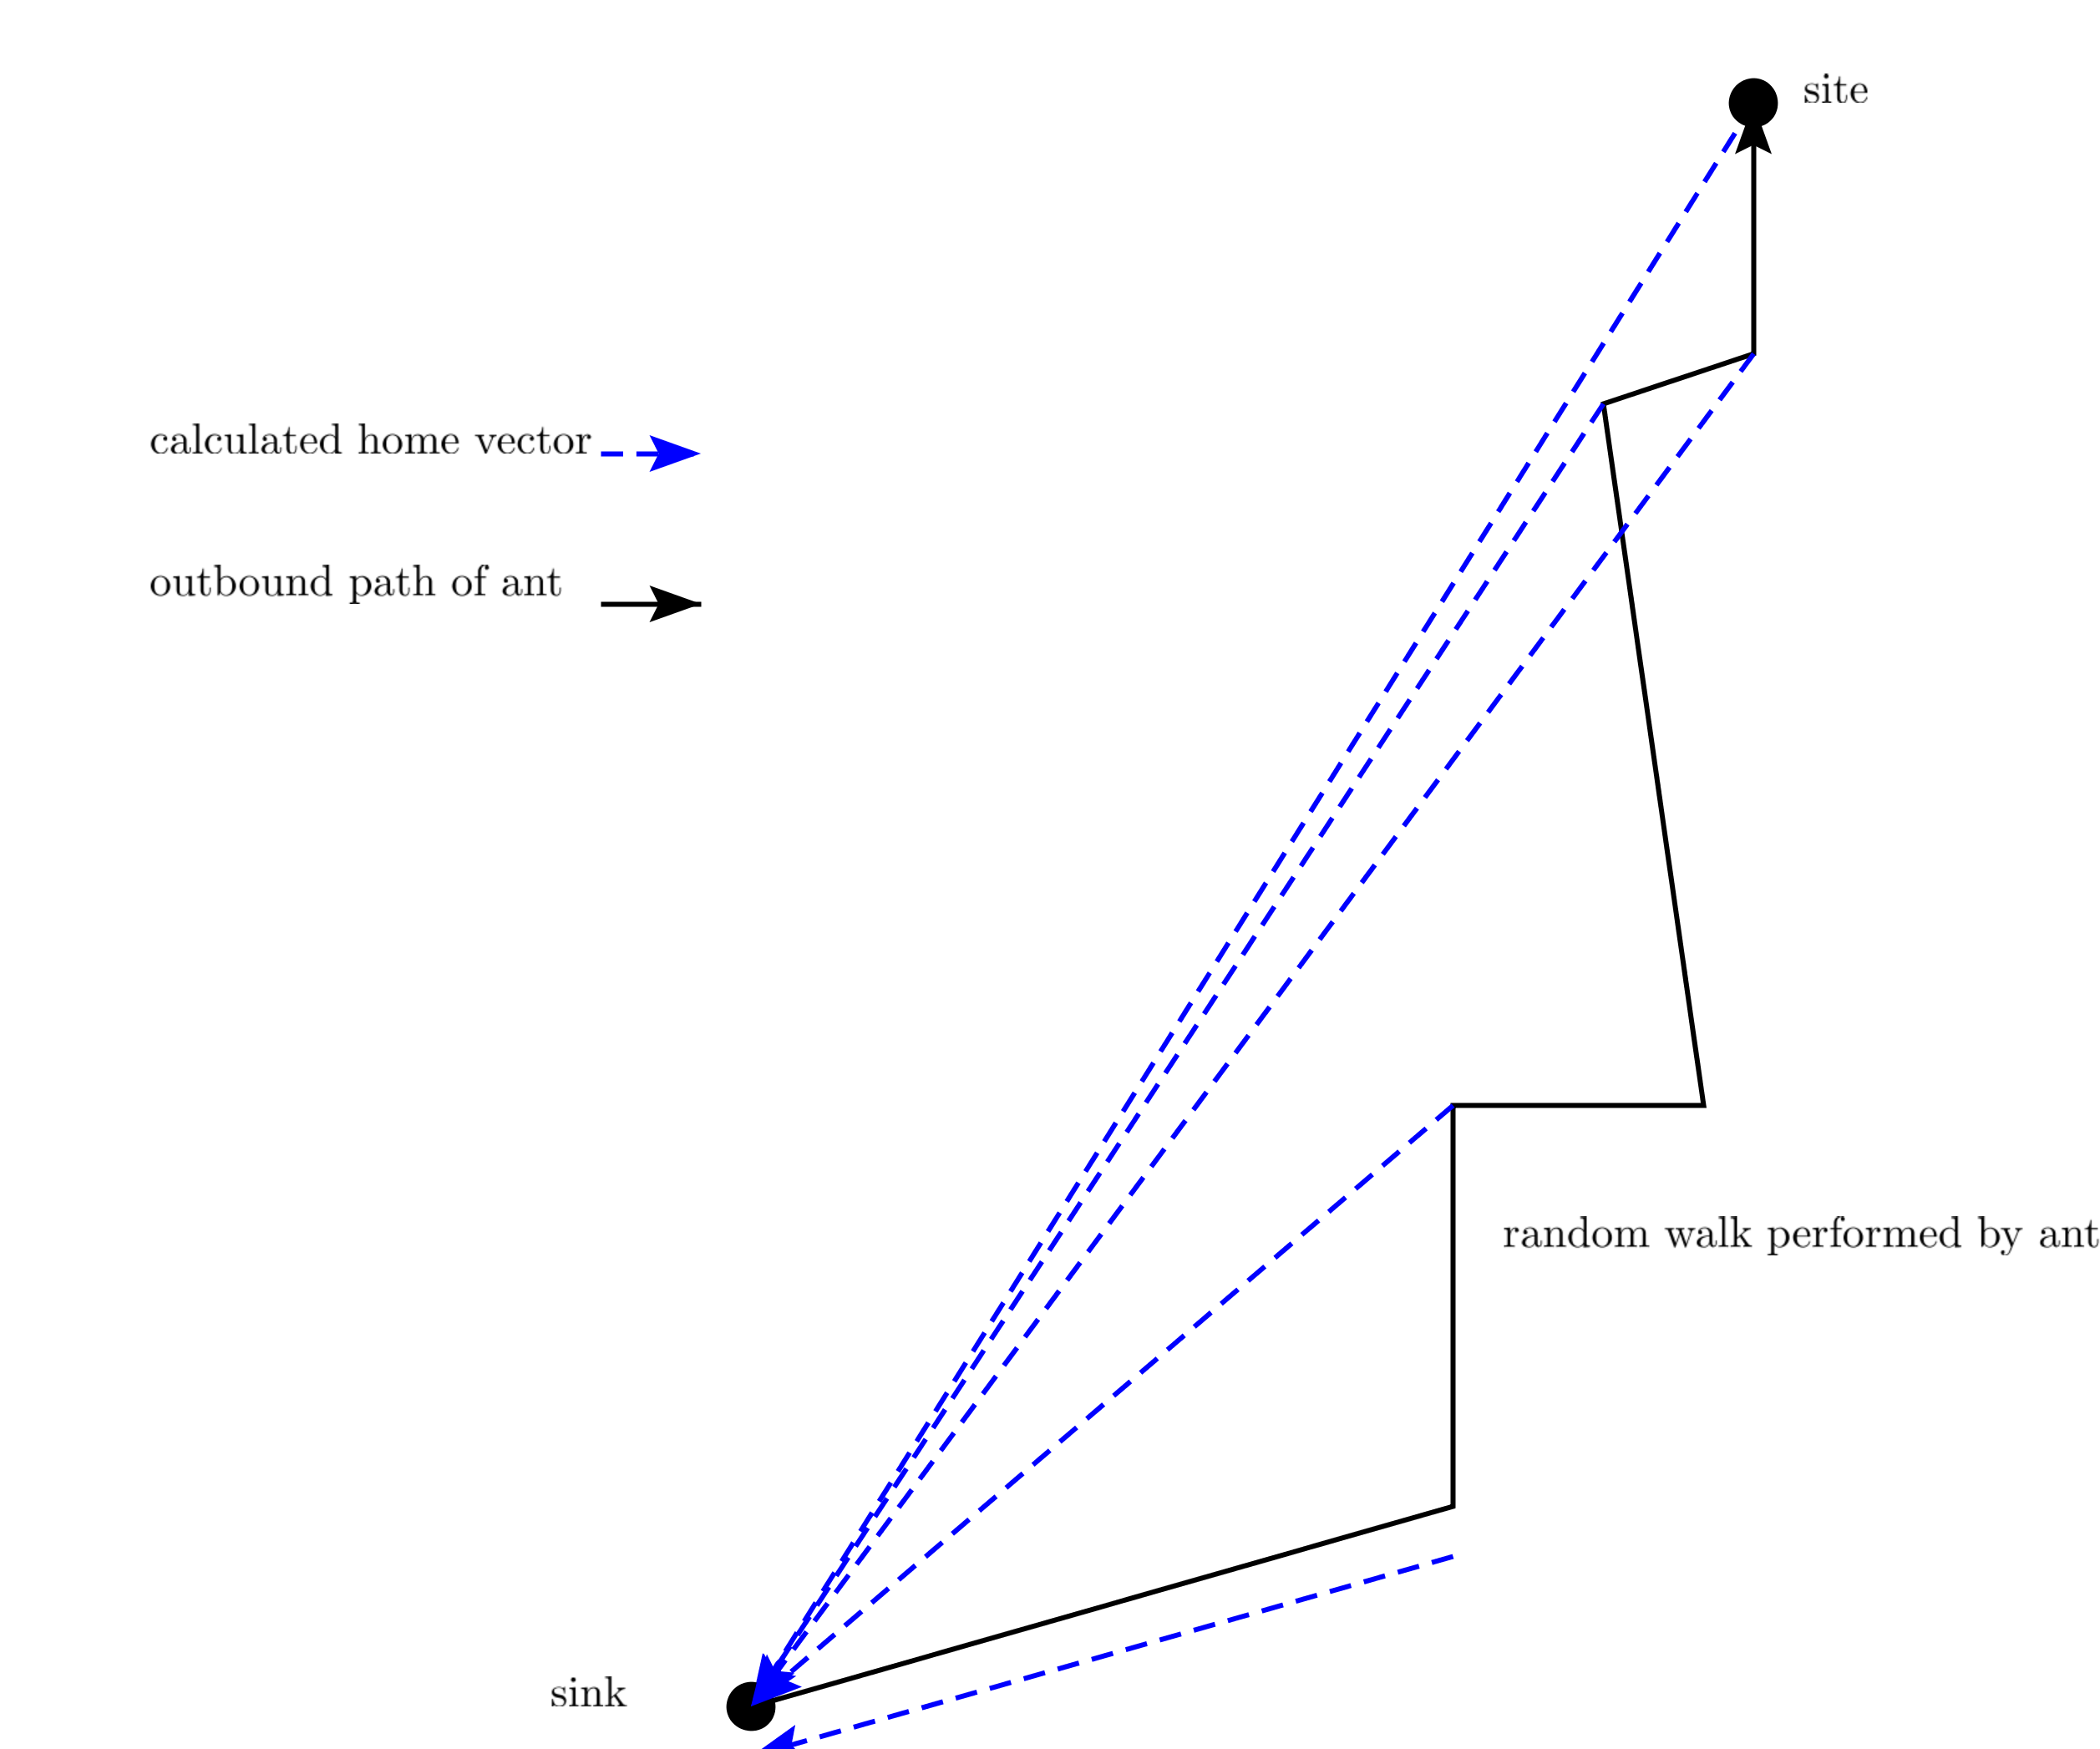
\includegraphics[width=\textwidth]{chapters/chapter2/figures/drawing.png}
	\caption{Path Integration }
	\label{pathintegration}
\end{figure}

Due to the lack of pheromone, the desert ant is thus simpler to model for real-robot interaction. Desert ant foraging has been modelled in \cite{moller1998modeling,hecker2012formica}. Hecker et al \cite{hecker2012formica} performed experiments to compare the performance of two foraging algorithms algorithms: The one algorithm was based on the desert ant foraging which has no pheromone-like communication and the other used including pheromone-like communication. It was shown that communication improved performance; however, the desert-ant algorithm still performed comparatively well. 

\subsection{Honey bee}
\label{honeybeeinnature}
Bees have an impressive set of abilities considering the simplicity of a single individual. They have the ability to remember the colour and shape of flowers \cite{zhang2006honeybee}, and in terms of navigation, they are able to learn local features and routes due to well-developed learning and memorizing capacities \cite{menzel2001cognitive}. Honey-bees are even time aware \cite{moore1989influence}. 

Honey bees have efficient division of labour between different functions in the hive, such as foraging and brood-care. Within the foraging activity itself, honey bees perform foraging-specific division of labours. Honey bee foraging is made up of three different roles namely employed foraging, unemployed foraging and scouting \cite{seeley2009wisdom}. Scouts explore the environment to locate new food sources. Once a source has been found, scouts return to the hive to communicate information about the located food source. To communicate the foraging information, scout bees perform a waggle-dance at the hive. The waggle-dance communicates information about the distance and bearing of the resource. The communication of a good foraging site is known as recruitment \cite{seeley2009wisdom}.

Unemployed foragers wait on the dance floor, and evaluate the dances of the scout bees. An unemployed bee select a location described by the scout bees, and become an employed forager. Employed forager bees use the information about the resource, attempt to locate the source, load themselves with food, and return to the hive where unemployed foragers are ready to offload the food. Jansen \cite{janson2007searching} suggests that unemployed bees become exploring scouts when they do not detect any dancing scout bees. 

\section{Types of Robot Foraging}
\label{sec:second:types}

Foraging is a popular problem due to the vast potential opportunity of foraging for application to a variety of real-world problems from search and rescue \cite{jennings1997cooperative} to toxic waste retrieval to mining. The foraging problem has been adapted by many swarm robotics resources into a variety of flavours of foraging. Thus it is beneficial to present a taxonomy of robot foraging that can be used to classify existing research about foraging as well as contextualize the specific foraging problems addressed by this thesis. Multiple taxonomies have been developed as robot foraging research has progressed \cite{oster1978caste,ostergaard2001emergent}. However a more recent and complete foraging taxonomy is presented in \cite{winfield2009foraging}. The taxonomy classifies foraging solutions based on four major axes: the foraging environment, the capabilities and types of robots used for foraging, performance aspects, and the foraging strategy used in a foraging algorithm. Each of these major axes have a number of minor axes which are outlined in Table~\cite{foragingtaxonomytable_part1}.  

The environment axis contains minor axes as follows:
\begin{itemize}
\item The type of search space which can be either unbounded or constrained by a boundary wall.
\item The type of objects in terms of whether they move (active) or not (static) and the quantity of objects (single or multiple).
\item The types of object sources that exist in the environment. A "single limited" source denotes that all objects come from the same source and the source as a limited capacity for objects. A foraging environment with a "single unlimited" source means that only one source exists and an unlimited number of items can be foraged from the source. A foraging environment can also have multiple sources.
\item The environment can have a single or multiple sinks
\item Objects can be placed in known locations, in a uniform distribution or in clusters in the environment.
\end{itemize}

The robot axis refers to qualities such as  the number of robots and the sensory, power and actuation capabilities of the robots. 
\begin{itemize}
\item Robots of the swarm can either be all identical (homogenous) or have different capabilities (heterogenous).  
\item The sensors of the robot can be of a limited range or  versus global sensors with unlimited range. 
\item Localization refers to the robots ability to position themselves in the environment. Localization could be non-existent, relative (such as path integration) or absolute (such as GPS).
\item Communication capabilities of the robots to each other can have infinite range, near range or not exist at all.
\item Robots can have an infinite power source, a limited power source, or a power source which can be sustained by foraging resources.
\end{itemize}

The performance axis characterises robot foraging on the methods used to evaluate the performance of a foraging algorithm, such as energy usage, or time taken to forage each item. Each minor axis described as follows:

\begin{itemize}
\item Performance of a foraging algorithm can be classified in terms of time taken to forage. A foraging experiment can be allowed infinite time to foraged, a fixed time for foraging or is attempting to minimize the time taken to forage
\item The energy that a robot can spend on foraging can be a fixed amount of energy, an unlimited amount of energy or a foraging algorithm can attempt to minimize the energy used to forage.
\end{itemize}

The strategy axis characterizes algorithms by the techniques that a foraging algorithm implements such as the type of search used or the type of recruitment technique used in a foraging algorithm. Each type of strategy is discussed as follows:

\begin{itemize}
\item The first stage of most foraging algorithm is the search for items. Search can occur in a number of ways. Foraging algorithms can be categorized in terms of their search technique such as: random search, following trails of items, following other robots, groups of robots looking for items together, where robots search in geometrical patterns and where search can only occur in a limited range of the sink.
\item Once an item is found it must be picked up. The techniques used by an algorithm for grabbing an item can be used to classify the algorithm. An item can be grabbed by a single robot or a group of robots can attempt to co-operatively grab an item.
\item Transport of an item back to the sink be performed by a single robot or by a a group of co-operating robots.
\item In order to get to the sink, a number of homing techniques can be used such as homing on a beacon, following a trail or self-navigation (such as path integration).
\item Robots can recruit other robots to forage certain areas. The technique for recruitment can be used to classify foraging algorithms. Direct recruitment is where a robot explicitly communicates to another robot to come forage an item source. Indirect recruitment is where a robot is recruited to forage by inexplicit communication from other robots (for instance, the number of robots waiting at the sink has increased above a threshold). 
\item Coordination between robots in a swarm can occur in a number of ways: there are can centralized control between all robots (not a true robot swarm), a master-slave configuration where one robot leads the others. Robots can be self-organized or can have no coordination at all. 
\end{itemize}

\begin{table}
\centering
    \caption{Winfield's Robot Foraging Taxonomy \cite{winfield2009foraging}}
    \label{foragingtaxonomytable_part1}
    
\begin{tabular}{ | c | c | c |}
	\hline
	Major Axis & Minor Axis & Value  \\ \hline
	\multirow{13}{*}{Environment}
		& \multirow{2}{*}{Search space} 
			& Unbounded \\  
		& 	& Constrained \\ \cline{2-3}
		& \multirow{3}{*}{Source Areas} 
			& Single limited \\ 
		&	& Single unlimited \\
		&	& Multiple \\ \cline{2-3}
		& \multirow{2}{*}{Sinks} 
			& Single \\
		&	& Multiple \\ \cline{2-3}
		& \multirow{3}{*}{Object types} 
			& Single static \\
		&	& Multiple static \\
		&	& Single active \\ \cline{2-3}
		& \multirow{3}{*}{Object placement} 
			& Fixed known locations \\
		&	& Uniform Distributions \\
		&	& Clustered \\\hline
	\multirow{16}{*}{Robot(s)}
		& \multirow{2}{*}{Number} 
			& Single \\  
		& 	& Multiple \\ \cline{2-3}
		& \multirow{3}{*}{Type} 
			& Homogenous \\ 
		&	& Heterogenous \\ \cline{2-3}
		& \multirow{2}{*}{Object Sensing} 
			& Limited range \\
		&	& Unlimited range\\ \cline{2-3}
		& \multirow{3}{*}{Localization} 
			& None \\
		&	& Relative \\
		&	& Absolute \\ \cline{2-3}
		& \multirow{3}{*}{Communications} 
			& None \\
		&	& Near \\
		&	& Infinite \\\cline{2-3}
		& \multirow{3}{*}{Power} 
			& Limited \\
		&	& Forage \\
		&	& Unlimited \\\hline
\end{tabular}
\end{table}

\begin{table}
\centering
    \caption{Winfield's Robot Foraging Taxonomy Part 2 \cite{winfield2009foraging}}
    \label{foragingtaxonomytable_part2}
    
\begin{tabular}{ | c | c | c |}
\hline
	Major Axis & Minor Axis & Value  \\ \hline
	\multirow{6}{*}{Performance}
		& \multirow{3}{*}{Time} 
			& Fixed \\  
		& 	& Minimum \\ 
		& 	& Unlimited \\ \cline{2-3}
		& \multirow{3}{*}{Energy} 
			& Fixed \\ 
		& 	& Minimum \\ 
		&	& Unlimited \\ \hline
	\multirow{6}{*}{Strategy}	
		& \multirow{5}{*}{Search} 
			& Limited range \\
		&	& Geometrical pattern\\
		&	& Trail following\\
		&	& Follow other robots\\
		&	& In teams\\ \cline{2-3}
		& \multirow{2}{*}{Grabbing} 
			& Single \\
		&	& Cooperative \\ \cline{2-3}
		& \multirow{2}{*}{Transport} 
			& Single \\
		&	& Cooperative \\ \cline{2-3}
		& \multirow{3}{*}{Homing} 
			& Self navigation \\
		&	& Home on beacon \\
		&	& Follow trail \\\cline{2-3}
		& \multirow{3}{*}{Recruitment} 
			& None \\
		&	& Direct \\
		&	& Indirect \\\cline{2-3}
		& \multirow{3}{*}{Coordination} 
			& None \\
		&	& Self-organized \\
		&	&  Central control \\
		&	& Master slave \\\hline
\end{tabular}
\end{table}


%%%%%%%%%%%%%%%%%%%%%%%%%%%%%%%%%%%%%%%%%%%%%%%%%

\section{Challenges in Foraging}
\label{challengesinforaging}
%TODO: Citations

Foraging for humans is a near trivial problem. Most children can walk around and retrieve blocks and return them to a single source. The seemingly simple sub-activities required by foraging such as identification and grasping are often relatively complex for robots to perform. Unlike other simpler, swarm robotics problems such as aggregation, foraging is made up of a group of non-trivial sub-tasks. Some of the aspects which are problematic for robots in a foraging are discussed below:

\begin{itemize}
\item Mechanically Challenging Interactions - Despite how far robotics has come as a field, there are still tasks that are trivial for humans, but still very complex for most robots. For instance, the challenge of picking up items \cite{saxena2008robotic} and moving them to another location requires high quality sensors, sensitive actuators and time-consuming calibration \cite{mondada2005cooperation}. 

\item Complex Noisy Environments - Although research can be performed in a controlled environment, for robust foraging to be efficiently applied in real-life, environmental factors have to be taken into consideration. Environmental factors such as light \cite{browning2005real,jungel2003real} and quality of the surface the robots forage on \cite{trianni2006cooperative}, often make a robotic solution complex, non-viable, non-robust or expensive. To cope with real-life environments, the robots require adaptive algorithms and more complex hardware for their sensors and actuators for basic navigation and object detection in unknown terrains with unknown lighting and weather conditions. 

\item Localization, Navigation and Obstacle Avoidance - Localization is the ability for a robot to depict their position in the environment. In swarm robotics, global knowledge about location (such as GPS) cannot be used by a robot to determine their position and where they are going. Non-trivial algorithms must be designed in order for a robot to position itself in the environment as ins \cite{zhou2012motion,rothermich2004distributed,arkin1992cooperation}. 

\end{itemize}

Swarm robotics researchers often choose to use simulated robot platforms such as Stage \cite{vaughan2008massively} or Argos \cite{pinciroli2011argos}, instead of real robots, in order to remove or regulate the amount of environmental noise. If a swarm robotics experiment uses real-life robots, the environments are usually simplified, by creating an environment where temperature, lighting and moisture are regulated\cite{labella2006division,nouyan2006group}. Due to the discussed complexities of foraging, existing swarm robotic research often simplifies the some of the complexities such as environmental changes, sensor noise, and the use of physical robots, in order to focus on a single aspect of foraging. 

\section{Foraging Algorithms}
\label{sec:second:existingsolution}

This section discusses some foraging solutions that have been developed as well as looks at the different types of foraging problems. 

Insects swarms are used as inspiration throughout swarm robotics due to their robust and flexible nature. Ants utilize pheromones which is a robust strategy for local interactions and would prove useful in hazardous environments. Section \ref{sec:second:natureinspired} discusses nature-inspired foraging algorithms while standard foraging algorithms are addressed in Section~\ref{standardforaging}. Section~\ref{multiforaging} discusses a more complex version of foraging with multiple object types. 
 
\subsection{Nature-inspired Swarm Robotics Foraging Algorithms}
\label{sec:second:natureinspired}

Foraging is an animal activity performed in order to retrieve food. Social insects in particular have found very efficient means of foraging despite their individual simplicity. The next few sections look deeper into algorithms that have been inspired by ant foraging, bee foraging and other aspects in nature. 

\subsubsection{Ant-inspired Foraging Algorithms}

%Blazing a trail => Nice paper - need to discuss more. Maybe in navigation
Vaughan presents a swarm robotic algorithm allowing for robust transportation of items from a single source to a single sink in an environment with spatial constraints \cite{vaughan2000blazing}. The algorithm presented makes use of both ant-like and bee-like foraging techniques. The ants broadcast the landmarks in the area for odometric localization as well as uses a form of the  honey bee "waggle dance" that communicates the direction of the food source from the robot that has found the food source to other robots. The robots use a technique called path integration utilized by both ants and bees in order to maintain position and heading estimate. Using these techniques the robots communicate multi-segment paths. These communications occur globally. This technique suffers from accumulation of localization errors over time due to the use of global communication. Local communication is preferred for the algorithms developed in this study.   %Our robot algorithms can reaign the sink %citations required!!!! %necessary? Worth a mention. 


%ANTS%
Hoff \cite{hoff2010two} classifies different types of ant-inspired pheromone-based foraging algorithms by how the pheromones are represented: physical marks \cite{alcoholfromants2012}, use of existing communication channels such as sharing over wireless networks as well as virtual pheromone. %Read further

%DoL in a Group of Robots Inspired by Ants Foraging Behaviour - Labella + Dorigo
Labella et al \cite{labella2006division} propose a foraging model inspired by the foraging of ants, where individual robots adapt to the environment using only locally available information. The adaption allows for effective division of labour to occur. The probability $p1$ that a robot will changed from rest to searching is adapted upon return to the sink and from deposit to rest. If a robot fails to forage any prey after searching for a specified maximum time, then the robot returns and rests. 
The adaption rule increases or decreases $p1$ by a constant $\Delta$ that is multiplied by the number of consecutive successes or failures. The study showed that adaption improved the amount of time spent not at rest. The advantage to this type of algorithm is its simplicity as no communication is required to regulate the number of robots. As pointed out, there is a global negative effect on overall efficiency at large group sizes. This is to be expected, but is not a serious problem since less energy is used, and this would be an advantage when energy is a scarce resource. %rephrase%
%Different from the problem proposed in this study as different priorities of items are not considered
%Come back and do a bit later. 
%Says prey

\begin{figure}
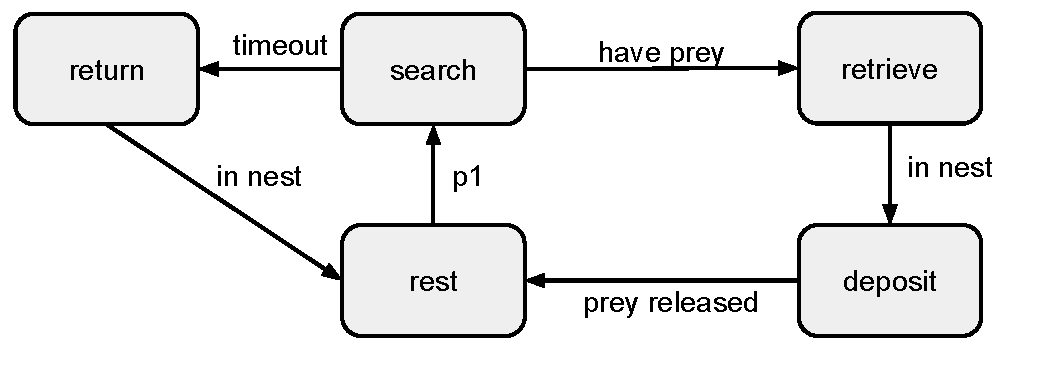
\includegraphics[width=\textwidth]{chapters/chapter2/figures/LabellaFSM.pdf}
\caption{Simplified finite state machine for Labella division of labour algorithm. }
\end{figure} 

Hoff \cite{hoff2010two} proposes a two ant-based foraging algorithm which do not require marking the physical environment. Instead, robots themselves become pheromone markers. The algorithms differ in the manner in which the beacon-to-pheromone role is chosen. 

Virtual pheromone algorithm functions as follows: Two pheromone trails are created - one trail from the source to the food and another trail from the source to the nest. The trail is created by robots: During execution, robots stop exploration and become pheromone beacons. The pheromone beacon robots simply broadcast a floating point number known as virtual pheromone. 
Local direct communications are used to transmit the virtual pheromone value.

The second technique uses cardinality where if a robot can hear 2 or more beacons then the robot stays a walker else the robot becomes a beacon. The advantage of using this technique over the other mentioned pheromone techniques is that robots are simpler due to simpler communication mechanisms as well as the lack of need for complex beacon deployment systems. Experiments are conducted with and without obstacles and a real-world simulator is used. The result show that congestion effects performance the most at high robot density. %write more in more detail. The cardin

\subsubsection{Bee-inspired Foraging Algorithms}
Bee swarms have been used in swarm robotics for problems such as path planning \cite{lin2009chaotic}, aggregation \cite{kernbach2009re}, collective perception \cite{schmickl2007collective}. Foraging algorithms have been developed that simulate a simplified honey bee recruitment in \cite{alers2014biologically}, which focuses on an actual robot demonstration of the technique using a turtle robot. Prior work focuses on implementing the same algorithm on e-pucks. 

The algorithm consists of two phases: an exploratory phase followed by an exploitive phase. Initially, all robots are located around the hive. In the exploratory phase, all robots perform a random search with a levy distribution until a food source is found by a robot. The exploitation phase begins where the robot that located the food returns to the hive and communicates the location to other members of the robot swarm. The other robots are recruited and begin to commute between the hive and the food source, transporting virtual food. This algorithm claims to exhibit three behaviours of bees: waiting around the hive, exploring the environment and foraging. Unlike bees, the algorithm used does not consider the division of labour between foragers, explorers and waiting robots, but rather uses an extremely simple model for bees which can only exploit a single food source. The robots use path integration in order to remember the location of the food source, and use a north-star type navigation in order to locate the hive. The path integration vector gets communicated to the other robots which use the vector to guide them to the food source. 

\subsection{Standard foraging}
\label{standardforaging}

%Fotan & Mataric
Schneider \cite{schneider1998territorial}, in order to reduce the interference caused by collisions, develop an algorithm to split the foraging environment into bounded areas for which a robot is in charge of. The sink area of one robot is the source area for the next, resulting in the emergence of bucket brigading behaviour. The bucket brigading algorithm is not suitable to environments where the size of the environment is not known - unless an algorithm is developed that will effectively allow a swarm of robots to divide the area. The algorithm is thus not suitable for comparison for the current study. The failure of a robot induces readjustment of territories in order to effectively cover the foraging area. Global information about the environment is used and as a result the algorithm is not suitable for comparison. %Reread to figure out if initial distribution algorithm exists

%Mataric
\O stergaard \cite{ostergaard2001emergent} determines that there is a finite number of any particular type of robot that is optimal for performing a foraging task. Mataric compares the algorithm to a naive algorithm which represents the baseline foraging task with no improvements. The naive algorithm in the thesis as a baseline comparison measure and is discussed in more detail in further chapters. Mataric found that if too many robots were allocated to the environment then extreme amounts of interference occurred which decreased the performance of the algorithm. Emergent bucket brigading was shown to perform better than naive in highly constrained environments however naive performed better in open environments. Algorithms are tested in environments of differing difficulties. %Need to read this paper to check which one these details came from. Also DO the thing for his name

%Goldberg + Mataric
Goldberg and Mataric \cite{Goldberg01designand} address the foraging problem with multiple sources and sink areas in an open field environment. The study focuses on interference reduction by making use of a dominance hierarchy - only the dominant robot near the sink can take an item to the sink. %mentioned PACK foraging. read up

%Mataric and Werger
Mataric \cite{werger1996robotic} and Werner discuss produced an algorithm where chains of robots are formed and the robots forage in circular excursions. The length of the change is then adusted according to the amount of food found by the foragers. %No idea how this works - read up. 
 
%Swarming Robots: Foraging Behaviour of Simple Multi-Robot System
Sugawara \cite{sugawara2002swarming} implements a foraging solution for a single food source. The algorithm is based on naive foraging however utilizes simple communication. A robot will stay and broadcast a light signal on finding an item. Other robots are attacted to the light signal based on an angular velocity equation. This differs from the techniques used in this thesis as all food sources communicated with equal weight where as the quality of a food source is evaluated by the honey bee algorithm.

%Alexandre Campo 2006 - Efficient multi-foraging robotics
\subsection{Multi-foraging}
\label{multiforaging}
Multi-foraging is defined as a type of foraging problem where instead multiple object types are required to be foraged. \cite{Balch99rewardand}. The types of objects can have different characteristics and can be collected together or separately.

%Adaptive DoL in Large-scale Minimalist MultiRobot systems - Mataric.
%2 types of items 
Jones et al \cite{jones2003adaptive} describe a version of the problem where there exist two types of items and items are consumed instead of transported to the sink and as items are consumed, the same type of item is placed at a random spot in the arena. Robots signal what type of item they are foraging by a coloured light which other robots use to build a local history of the number of robots they have seen that are allocated to each item type. A history of the number of observed items of each type is also collected. The division of labour capability is formed by estimating the current division of labour of the group by  using the described local observations. The estimations are then used to determine the probability of changing from foraging the current item type to the other type. 

%\begin{equation}
% P(Green - Red) = \left\ {
%	\begin{array} {l l}
%		(GR - GP_*(1-GP) & \quad \textrm{if GR \geq GP} \\
%		0, & \quad \textrm{otherwise}
%	\end{array}
% \right.
%\end{equation} 

%		(RR- RP)*(1-RP) & \quad \text{if RR $\geq RP$
%%%%DoL$
Campo \cite{campo2007efficient} performs a study in order to identify characteristics of efficient multi-foraging behaviour.  A mathematical model is developed and validated to predict optimal foraging behaviour and thus allows absolute evaluation of the proposed decision algorithm. The proposed foraging decision algorithm utilizes the amount of other robots encountered as well as the amount of prey encountered to only allocate enough robots foraging  so that remaining robots can spare energy. A measure is proposed that estimates the instantaneous energy that a robot group can gain, which each robot uses to guide the search process. 
%Need to add discussion
%Says prey

Balch \cite{balch1999impact} develops a technique for multi-foraging and determining the impact of robot diversity on multi-foraging performance. This thesis's does not consider robot diversity since robots are homogenous.

%%%%%%%%%%%%%%%%%%%%%%%%%%%%%%%%%%%%%%%%%%%%%%%%%
%%%%%%%%%%%%%%%%%%%%%%%%%%%%%%%%%%%%%%%%%%%%%%%%%


\section{Prioritized Foraging}
\label{sec:second:prioritizedforaging}

%Focus on the robots used, the model used and the experiments performed

The multi-foraging problem is a more complex version of standard foraging, where more than one type of item must be foraged to a separate sink \cite{balch1999impact}. That in mind, the prioritized foraging problem, shown in Fig.\ref{prioritizedforaging}, is defined as a modified version of the multi-foraging problem where an environment has two types of items: prioritized items and non-prioritized items. The goal is to forage all the items of the prioritized type. The possibility exists that prioritized items become trapped among non-prioritized items and thus the non-prioritized items need to be removed from the environment to clear an access route to the prioritized items. 

The prioritized foraging problem has increased difficulty due the fact that  foraging the non-prioritized item more than required will result in a waste of time and energy. The goal of research in prioritized foraging is to develop an algorithm to efficiently adapt the number of robots searching for prioritized items to those moving non-prioritized items out the way. 

The prioritized foraging problem is suitably applied to search and rescue. For example, in the case of a building collapsing, robots will need to get to the survivors as quickly as possible, however it is important that some robots move waste material in order to reach the trapped survivors. Prioritized foraging could be applied to the gold mining problem where the gold needs to be foraged as a priority and the waste needs to be moved out the way.


\begin{figure} [h]
	\centering
	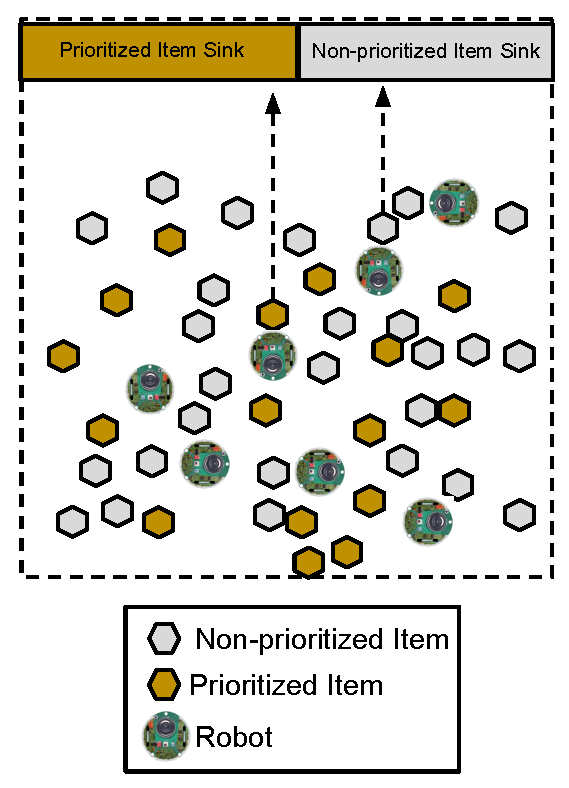
\includegraphics[width=0.65\textwidth]{chapters/chapter2/figures/EpuckGoldMining.pdf}
	\caption{Prioritized Foraging Problem }
	\label{prioritizedforaging}
\end{figure}

As per Winfield's classification described in section \ref{sec:second:taxonomy}, the prioritized foraging problem has a constrained environment, multiple source areas with multiple sinks, multiple object types, object placement is tested in a number of environment types explained in the following sections. There are multiple homogenous robots with limited sensing, relative localisation with near communications and unlimited power. Power is kept as unlimited since the energy preservation of algorithms is to be studied as a performance measure. 

%%%%%%%%%%%%%%%%%%%%%%%%%%%%%%%%%%%%%%%%%%%%%%%%%
%%%%%%%%%%%%%%%%%%%%%%%%%%%%%%%%%%%%%%%%%%%%%%%%%
\section{Summary}
\label{foraging:summary}

This chapter focused on reviewing foraging in nature and in swarm robotics as well as presenting a novel form of the foraging algorithm called prioritized foraging. 

In nature, social insects have efficient emergent foraging behaviours. Ants generally lay pheromone to guide the item search process, but the desert ant does not use pheromone and thus use a technique called path integration to relocate a food source. Honey bees employ more complex foraging behaviour including division of labour and communication. Winfield's foraging taxonomy is presented and discussed so that research can be contextualized in the field. 

Existing swarm robotics foraging algorithms are addressed and discussed under three sections: nature-inspired algorithm, standard foraging algorithms and multi foraging algorithms. Lastly, the novel idea of prioritized foraging is introduced. In prioritized foraging a particular item type has higher priority than other items. 

\chapter{Division of Labour}
\label{chap:divisionoflabour}

Due to the importance of division of labour in this research, a variety of division of labour strategies from social insects should be highlighted, explored and contrasted. This chapter defines division of labour as well as analyses different types of division of labour that occur in social insects. Lastly, division of labour strategies employed by different swarm robotics algorithms are employed. 

\section{Definition}
\label{sec:second:definition}

Oster et al. defines division of labour as a "stable pattern of variation" among individuals within a swarm in terms of the repertoire of tasks that individuals perform where each individual specializes on a subset of the complete repertoire of tasks performed by the swarm and the subset of tasks varies across individuals in the swarm \cite{oster1978caste}.  
More simply, Robinson et al. define division of labour as the adjustment of ratios of workers engaged in different tasks based on external and internal stimuli \cite{robinson1992regulation}.

There are two types of division of labour in social insects: 
\begin{itemize}
	\item Temporal polyethism - The pattern of tasks being performed by a worker correlates to the age of the worker. In nature, the younger workers may perform tasks within the nest while the older workers perform tasks outside of the nest.
	\item Morphological polyethism - A worker with some extreme features in terms of size or shape, will specialize more in particular tasks and the more extreme that feature is, the narrower the repertoire of the of the worker. In nature, for example, larger workers would be more likely to form part of defence of the nest. \cite{beshers2001models}
\end{itemize}

%NEED SOMETHING HERE

%include if we find we need. for now, you're done
%\subsubsection{Task Selection}
%Before addressing the different models of division of labour, it's important to discuss one of the main distringuishing characteristics of division of labour: How does an individual select tasks? Much of the study of division of labour is related to how workers select tasks. The factors contributing to the decision are divided into internal and external factors. Internal factors refer to neurological, hormonal, experience or genetic factors where as the external factors refer to environmental stimuli, worker to worker interaction and communication of the increasing need of workers assigned to a particular task. \cite{beshers2001models}.

%Research around task selection is focused around the following topics: 
%\begin{itemize}
%	\item The rules guiding the decision process in workers
%	\item The process of how information about the environment and social stimuli is gathered
%	\item The internal choice mechanism for making the decisions
%\end{itemize}

\section{Models of Division of Labour from Biology}

Beshers at al \cite{beshers2001models} provide a extensive overview of models of division of labour in insects. Due to the use of insect division of labour addressed by algorithms developed in this thesis, an overview of existing models is provided in the next section.

\subsection{Response Threshold Model}

In the response threshold model, workers have intrinsic thresholds for reacting to task-specific stimuli. The variation in task thresholds among workers in a swarm induces the division of labour \cite{robinson1992regulation}. The response threshold model identifies variation in the worker environment interaction as the primary reason for division of labour

Each task in the repertoire has a related response threshold. The default state of all workers is to have no task assigned. All workers have some threshold for a task and higher stimulus levels result in recruitment of additional workers into a task group. Specialist have the lowest thresholds for a particular task. A negative feedback loop is formed because as the performance of a task by a worker increases, the stimulus level of that task decreases. If a worker with a lower threshold reaches a task then the worker with the higher threshold may never reach that threshold and thus will never perform the task \cite{beshers2001models}.

The simplicity of the response threshold model makes it a popular choice for division of labour in swarm robotics, however it suffers from a number of problems. A predominant problem is that a small intrinsic variation in the performance or responsiveness of a workers' ability to complete task may be amplified into large differences in task repertoire or the frequency of task performance. 

The response threshold model makes the assumption that all workers are equally likely to encounter each task and that stable equilibrium is reached when the number of workers performing a task matches the stimulus level and when individual workers maintain constant task performance probabilities \cite{page1990self}.

\subsection{Integrated Threshold--Information Transfer Model}
\label{integratedthreshold}

Integrated Threshold Information Transfer model can be discerned from it's name. Workers perform a task when the stimulus they encountered equals an internal threshold - the internal threshold will vary according to genetics. The process of discerning a task stimulus is known as information transfer. Information transfer can be perceived randomly in space, directly or via social information transfer  \cite{fewell1999division}. In Integrated Threshold-Information Transfer, both the integrated threshold can be varied as well as the method of transferring information.

Fewell et al  use information transfer models to predict swarm level response patterns to graded changes in stimulus levels for the tasks. The model predicted that normally distributed patterns of task thresholds would induce a graded response - independently of how the individuals received information about the task \cite{fewell1999division}.

%NOT VERY GOOD BUT FUCK IT!

\subsection{Foraging for Work}

Foraging for work is controversial in the fact that it induces division of labour without any explicit worker mechanism but instead a natural result of the environment \cite{beshers2001models}.  
Foraging for Work has two main parts:
\begin{enumerate}
	\item Workers repeat the same task when possible.
	\item Workers actively seek work when they have no task.
\end{enumerate}

%This forms the basic model of foraging and also is used in MY honey bee algorithm.

Foraging for work makes the assumptions that workers are intrinsically identical and thus task performance of workers is dependent on opportunity, rather than intrinsic task preferences. However, it has been shown that in true insect colonies, there is intrinsic variation in each worker's response to the environment as not all workers will respond equally. Another assumption is that tasks are radially spatially localized within the nest. That means the tasks further away are performed by older workers and the younger workers will perform the tasks that are nearer.

Foraging for work shows that temporal polyethism doesn't require age-related difference in the mechanism of task choice and can simply stem from the older workers proximity to the nest which is controversial as it sets the base expectation of what level of task organization might occur within a social group in absence of selection efforts or intrinsic mechanism of worker task performance \cite{franks1994foraging}.

Foraging for work can be seen as a special case of the threshold model where all workers have identical thresholds. The observation of this fact is that with Foraging for Work, temporal polyethism is generated by spatial organization, where as in threshold models polyethism is generated by differences in performance threshold. A disadvantage of threshold models is that lazy workers can be generated by those workers with high thresholds resulting in inactive workers where as according to Foraging for work all workers should either be performing or seeking tasks.

\subsection{Self Reinforcement Models}
\label{selfreinforcement}

Task success is directly proportional of the probability of doing the task again. Self reinforcement models answer the question about whether division of labour is generated as a result of experience \cite{lerman2005review}. If a task was not performed successfully or there was the lack of opportunity then the probability of ever performing that task reduces. The result is that task specialists are created. 

A study performed on foraging specializations by Deneubourg et al shows that self-reinforcement paired with worker age variation are to account for temporal polyethism \cite{deneubourg1987self}. Plowright and Plowright use self-reinforcement to generate elitism \cite{plowright1988elitism} determining that the result was a bimodal frequency of performing tasks where the agents either became specialists or became entirely inactive.

Theraulaz introduces the concept of learning and forgetting \cite{theraulaz1998response}. Learning is when there is a reduction in response threshold when a worker performs a task. And forgetting is an increase in response threshold when a worker doesn't perform a task. All individuals begin with equal thresholds. Evidence from the model indicated that workers adequately adjusted activity levels according to the task they ended up specializing in and exhibited flexibility such that when workers of a specific task are removed the swarm would adapt in order to cater for for missing individuals. 

%  /$$$$$$  /$$$$$$$$ /$$$$$$  /$$$$$$$ 
% /$$__  $$|__  $$__//$$__  $$| $$__  $$
%| $$  \__/   | $$  | $$  \ $$| $$  \ $$
%|  $$$$$$    | $$  | $$  | $$| $$$$$$$/
% \____  $$   | $$  | $$  | $$| $$____/ 
% /$$  \ $$   | $$  | $$  | $$| $$      
%|  $$$$$$/   | $$  |  $$$$$$/| $$      
% \______/    |__/   \______/ |__/      
%NB: ABOVE is what happens in my own things
                                   
\subsection{Network Models of Task Allocation}

Network models of Task allocation, developed in \cite{gordon1992parallel} and extended upon in \cite{pacala1996effects} are a model of simple interactions between workers. It assumes that workers are identical and instead division of labour is induced directly by effective communication of the number of workers required per task between workers. 
 
In this particular network allocation models a worker performs one of four tasks, where for each task they are either active or inactive. This results in each worker having 8 states. Workers having the same states belong to the same task group and all worker interactions are bias towards transferring information with workers that belong to the same task group \cite{gordon1992parallel}. The worker behaviour in each iteration is determined by a linear combination of interactions. The system moves to a balance of active and inactive workers. 

Pascala \cite{pacala1996effects} developed a differential equation to investigate the effects of social group size on task allocation. Information was received directly from the environment, through success or failure of task performance and random encounters with other group members. It was shown that large networks (ie a large number of agents) track environmental changes more efficiently as there is a higher rate of information flow but interaction increases substantially causing interference. Thus as colony size increases, the overhead from interactions becomes faster than the information collection rate from the environment. The solution is to limit the frequency of interaction \cite{pacala1996effects}

The key similarity between network models and foraging for work models is that despite the fact that goals differ, they both share the view that division of labor can be generated by changes in local information encountered by an individual worker. Local information is affected by availability of performance of other tasks, resulting in workers switching between task spaces. Network models are more accurate than the linear model of foraging for work, but network model lacks self organizational properties of foraging for work models.

\subsection{Social Inhibition Models}

The sheer presence of older foraging bees affects behavioural development as the proportion of bees becoming foragers is indirectly related to the number of older bees present in the swarm \citation{huang1992honeybee}. This effect is modelled in the activator-inhibitor model.

Activator-Inhibitor model is driven by 2 hormones:
\begin{itemize}
	\item The activator hormone which is the juvenile hormone that motivates the workers in the hive to become foragers.
	\item The inhibitor hormone which is transferred from the foragers to the younger workers, suppresses the bees development into foragers. If foragers are lost in an accident then more hive workers will mature to foragers due to the decrease of the level of the inhibitor hormone.
\end{itemize}

The mathematical version of the social inhibition model represents the workers physiological state by a single variable $x$ that changes daily in response to the social environment \cite{beshers2001social}. The model defines the trajectories for behavioural development that is intrinsically determined and responsive to social environments. Task performance is correlated with age. Social inhibition provides mechanism of changing worker thresholds as they age which response thresholds fail to do. Social inhibition models allow swarms to flexibly respond to dynamic environments. %pointsless but fuck it!%

\section{Division of Labour in Robot Swarms}

Numerous division of labour strategies have been used in robot swarms. Labella et al. \cite{labella2006division} develop a division of labour strategy for prey retrieval based on Deneubourg's ant self re-enforcement model as discussed in \ref{selfreinforcement}. Experimentation was performed on real robots as well as in simulation. Robots change from search to rest with probability $p$. This probability gets incremented when a robot successfully returned to the nest with an item and decremented when a robot returns to the nest without an item. They classified the foragers into different types based on the final value of $p$ - loafers, foragers and undecided and showed that the values of $p$ tended towards extremes showing that in general, robots tended to become either loafers or foragers, while only a few became undecided. It was shown that a simple self-reinforcement division of labour model can improve the performance of a swarm of robots at a task without the need for communication, however scalability is still a concern as there are negative effects as group size increases. In the author's opinion, this shows that division of labour is not entirely effective since algorithm able to to effectively divide labour would decrease the number of robots performing a specific task if there are too many robots performing the task.

Agassounon et al. design and demonstrate three threshold-based methods for division of labour\cite{agassounon2002efficiency} on clustering a number of small objects in order to dynamically allocate the most appropriate number of robots to the task. The idea is that initially there will be multiple possible sites for clustering, however later in the clustering process, having too many robots competing for a single site will cause interference decreasing the efficiency of the process. The experiment determined that the swarm benefited from threshold division of labour since the algorithms with division of labour performed similarly or better than those with a fixed group size. 

\begin{itemize}
\item The first algorithm, PrFT, does not use explicit communication and assigns fixed response thresholds to the robots.
\item The second algorithm, PrVT, does not use explicit communication and assigns variable response thresholds to each robot. 
\item The final algorithm, PuFT, makes use of explicit peer-to-peer communication between robots to communicate the worker demand but assigns fixed response thresholds to the robots.  Communication occurs when robots are in each other's communication range. The final worker threshold is calculated by averaging the worker threshold's from all robots in the communication range with their own sensed worker threshold. 
The PuFT algorithm is an example of Integrated Threshold -- Information Transfer as described in section \ref{integratedthreshold}.
\end{itemize}

In conclusion, the study determined that after a priori optimization of the fixed thresholds the algorithms performed comparatively similarly. PuFT appeared to perform the best, however the cost of communication was not included in the study. This result can possibly be attributed to the fact that information transfer increased the spread of environmental knowledge and thus the speed at which the division of labour parameters were adapted. Both fixed threshold algorithms suffered badly in environments where they were not optimized for. They pose that an algorithm combining the advantages of threshold variability and information sharing would be worth exploring. 

Liu et al. \cite{liu2007towards} introduce 3 mechanisms for adapting the number of resting robots to foraging robots in a simple foraging problem. The mechanisms consist of variations on how one perceives the worker demand: internal success at task, collective success at task and environmental interference while performing a task - specifically collisions with other agents. The algorithms modify time specific thresholds of how long to wait before going back to work and how long to work for. Four combinations of these factors are evaluated as well as compared to a nai\"ve foraging approach. The efficiency of the swarm is evaluated and compared at different food densities and robot quantities and evaluate energy spend as an efficiency metric rather than number of items foraged over time. %results

To conclude, it appears majority of existing division of labour research is focussed on determining the most efficient number of foragers that should be active at a time. The discussed division of labour strategies have been found to be seemingly beneficial in the problem of regulating the number of robots and despite the seeming simplicity of the problem - to perform a single task or not, the ability to regulate the number of robots is a key requirement of a swarm robotics system as it affects the flexibility, and scalability of a swarm. The ability to adjust the number of resources required to handle a particular problem results in an swarm with the ability to adapt to dynamic environments and thus increasing overall flexibility of the swarm. It also allows the performance to not degrade when more agents are added to the problem since robots will be able to adequately adjust when too many robots have been added and are decreasing productivity and efficiency. 

That said, there is space for addressing other types of division of labour and task allocation problems besides that of optimal number of active robots as many systems require division of labour between multiple active tasks. There is also a lack of implementation of other types of division of labour models such as the network based models which may be worth exploring.

Lastly, despite the general attempt to test scalability, the maximum swarm size is usually 10 or less. It is in the author's opinion that it would be beneficial to attempt this study on a larger scale problem with larger swarm sizes to truly see the benefit in the division of labour strategy to regulate the number of foraging robots. 

\section{Summary}
\label{sec:second:summary}
Division of labour is the adjustment of ratios of workers engaged in different tasks based on external and internal stimuli. Division of labour is used in social insect societies such as bees and ants and multiple models for division of labour have been explored by biologists. Extensive research has been performed about response threshold models, internal threshold information transfer, foraging for work and self-reinforcement models. The different models are explained and compared. Despite the large number of models, little verification of these models have been performed in real or simulate environments. 

Lastly, the use of division of labour in swarm robotics is explored. Most of the reviewed research was focused around the problem of using division of labour to regulate the number of active robots where a robot has two division of labour states - either actively performing the task or resting. The techniques used in swarm robotics employ a variety of division of labour models. The author notes that the reviewed research did not adequately address the scalability of the techniques and discussed how more complex version of division of labour problems still need to be addressed. % rename as required (but remember to update directories appropriately)
%%%%%%%%%%%%%%%%%%%%%%%%%%%%%%%%%%%%%%%%%%%%%%%%%
%%%%%%%%%%%%%%%%%%%%%%%%%%%%%%%%%%%%%%%%%%%%%%%%%

\chapter{Nature inspired algorithms for prioritized foraging}
\label{chap:third}

%%%%%%%%%%%%%%%%%%%%%%%%%%%%%%%%%%%%%%%%%%%%%%%%%
%%%%%%%%%%%%%%%%%%%%%%%%%%%%%%%%%%%%%%%%%%%%%%%%%

This chapter presents a foraging variation known as prioritized foraging as well as three algorithms whose performance is to be evaluated on a prioritized foraging problem. The three algorithms are based based upon phenomena observed in nature. The first model is a simple foraging algorithm, called na\"ive foraging, which will form the benchmark algorithm for the experiments. Two novel swarm robotics foraging algorithms, inspired by the foraging behaviour of desert ants and honey bees, are also presented. Each of these algorithms have different capabilities when it comes to memory, communication, division of labour, and navigation. The na\"ive foraging algorithm is presented in Section~\ref{naiveforaging}. Section~\ref{desertantforaging} introduces the novel foraging algorithm based on desert ants. Section~\ref{honeybeeforaging} presents a novel prioritized foraging algorithm inspired by honey bees. The algorithms are summarized in Section~\ref{prioritized:summary}.
%%%%%%%%%%%%%%%%%%%%%%%%%%%%%%%%%%%%%%%%%%%%%%%%%
%%%%%%%%%%%%%%%%%%%%%%%%%%%%%%%%%%%%%%%%%%%%%%%%%

\section{Prioritized foraging}
\label{sec:second:prioritizedforaging}

%Focus on the robots used, the model used and the experiments performed

The prioritized foraging problem, illustrated in Fig.\ref{prioritizedforaging}, is a modified version of the multi-foraging problem as discussed in Section~\ref{environmentaxis}. In prioritized foraging, an environment has two types of items: prioritized items and non-prioritized items. The goal is to forage all the items of the prioritized type. The possibility exists that prioritized items become trapped among non-prioritized items and thus the non-prioritized items need to be removed from the environment to clear an access route to the prioritized items. 

The prioritized foraging problem has increased difficulty compared to traditional multi-foraging problems, due the fact that foraging the non-prioritized item more than required will result in a waste of time and energy. The goal of research in prioritized foraging is to develop an algorithm to efficiently adapt the number of robots searching for prioritized items to those moving non-prioritized items out the way. 

The prioritized foraging problem has similarities to the problem of search and rescue. For example, in the case of a building collapsed, robots will need to get to the survivors as quickly as possible. However, it is important that some robots move waste material in order to reach the priority trapped survivors. Prioritized foraging could be applied to the gold mining problem where gold needs to be foraged as a priority, and waste needs to be moved out of the way.


\begin{figure} [h]
	\centering
	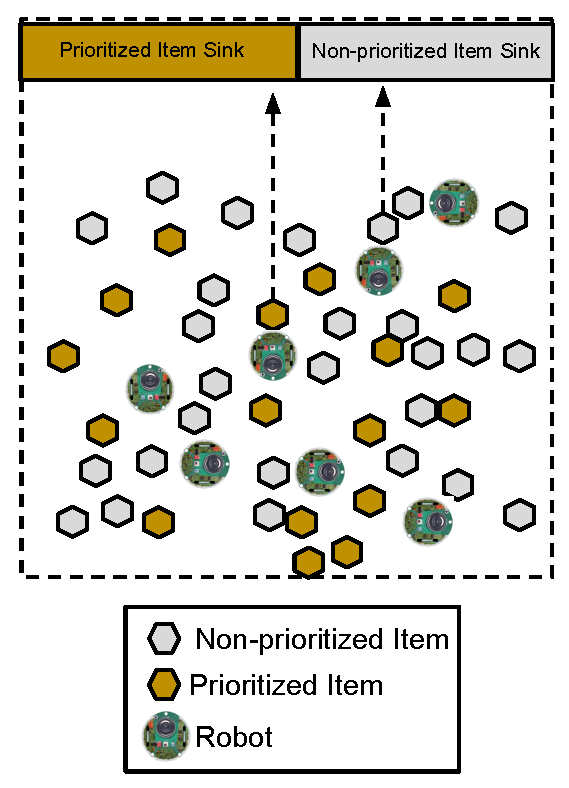
\includegraphics[width=0.65\textwidth]{chapters/chapter2/figures/EpuckGoldMining.pdf}
	\caption{Prioritized Foraging Problem }
	\label{prioritizedforaging}
\end{figure}

As per Winfield's classification discussed in Section~\ref{sec:second:taxonomy}, the prioritized foraging problem has the following characteristics: The environment has a bounded search space, with multiple source areas for items which can be placed in multiple sinks. Multiple object types exist in the environment - the prioritized items and the non-prioritized items. The primary  performance measure for the prioritized foraging problem is time, in terms optimizing the time taken to forage each type of item. 


\section{Na\"ive foraging algorithm}
\label{naiveforaging}

Na\"ive foraging consists of the following tasks: searching for an item, grabbing an item, returning home with the item, and storing the item at the sink. The steps performed by the algorithm are illustrated in Figure~\ref{naiveforagingstatediagram}, and described below:  

\begin{enumerate}
	\item Robots perform a random walk until they find an item.
	\item On locating an item, the robot grips the item. If the item has been moved before the robot is able to pick it up, the robot will continue to explore; otherwise, the robot returns the item to the correct sink using a beacon-based homing algorithm.
\end{enumerate}

\begin{figure} [h]
	\centering
	\begin{tikzpicture}[node distance=8cm]
	\node (randomwalk) [process] {random walk};
	\node (offload) [process, below of=randomwalk, yshift=4cm] {off-load};
	\node (loaditem) [process, right of=randomwalk] {load item};
	\node (homing) [process, right of=offload] {homing};
	\draw [arrow] (randomwalk) -- node[anchor=south] {locates item} (loaditem);
	\draw [arrow] (loaditem) -- node[anchor=west] {successful load} (homing);
	\draw [arrow] (homing) -- node[anchor=north] {at sink} (offload);
	\draw [arrow] (offload) -- node[anchor=west] {successful offload} (randomwalk);

	\draw[arrow,postaction={decorate,decoration={text along path,reverse path,raise=1ex,text align=center,text={unsuccessful load}}}] (loaditem) to[bend right=45] (randomwalk);
	\end{tikzpicture}
	\caption{Nai\"ve Foraging State Diagram}
	\label{naiveforagingstatediagram}
\end{figure}

Na\"\i ve foraging includes only the most minimal set of foraging actions and is included as a baseline for comparison to evaluate how novel techniques, such as the desert-ant foraging or honey-bee foraging, compare to a standard model \cite{ostergaard2001emergent,hoff2010two}.

The following random walk is used: A robot chooses a random direction, $\sigma$, and a random distance $m\in(0,M)$ where $M$ is a chosen maximum path length. The robot walks in direction $\sigma$ for distance $m$, or until the robot reaches a boundary. The robot then chooses new values for $\sigma$ and $m$.


\section{Desert ant foraging}
\label{desertantforaging}


As discussed in Section~\ref{biological:ants}, desert ant foraging behaviour is a very suitable model for robot foraging, since no pheromone depositors or pheromone mimickry is required. Pheromone depositors or pheromone mimickry are quite complex to perform in robot environments. Instead of pheromone, desert ants use path integration (PI) to memorize the location of an existing food source and later to return to the memorized source to find more food, as discussed in Section~\ref{biological:ants}. The notion of returning to a previously explored site is known as site fidelity \cite{switzer1993site}. The desert ant algorithm does not require communication between robots or the dispersal of beacons, and is thus simpler than many other swarm robotic foraging algorithms. The desert ant foraging robots can be in the following states:

\begin{enumerate}
	\item\textbf{Exploration State}: A robot in the exploration state performs a random walk with PI. The random walk used is the same random walk as discussed in Section~\ref{naiveforaging}. The purpose of the exploration state is to explore the environment to locate items. 
	\item\textbf{Loading State}: On finding an item, the robot switches into the loading state. In the loading state, the robot loads the item and memorizes the current PI vector. The PI vector is memorized so that the robot can use it to return to the sink and then later to return to the site where the item was found. If loading of the item fails (perhaps due to another robot loading the item), then the robot returns to the exploration state; otherwise, the robot moves into the homing state.
	\item\textbf{Homing State}: In the homing state, the robot uses the PI vector to move to the sink. The use of the PI vector will enable the robot to follow the most direct route back to the sink.
	\item\textbf{Offloading State}: When the robot arrives at the sink, the robot switches into the offloading state, where the robot simply offloads the item into the sink. 
	\item\textbf{Locating State}: Once the robot has offloaded the item, the robot switches to the locating state. In the locating state, the robot follows the memorized PI vector to the location of the previous item. The premise of returning to the site where the previous item was found is that more items may exist where the previous item was located in order to locate more items. If another item is found, the robot moves into the loading state; otherwise, the robot returns to the exploration state in the search of new items. 
\end{enumerate}

All robots begin at random positions adjacent to the sink in the exploration state. The desert ant foraging states and transitions are illustrated in Figure~\ref{fig:desertantstate}.

\begin{figure} [h]
	\centering
	\begin{tikzpicture}[node distance=6cm]
	\node (explorationstate) [process] {explore};
	\node (loadstate) [process, right of=randomwalk] {loading};
	\node (homing) [process, below of=loadstate,yshift=2cm] {homing};
	\node (offload) [process, left of=homing] {offload};
	\node (locating) [process, left of=explorationstate] {locating};
	\draw [arrow] (explorationstate) -- node[anchor=south] {locates item} (loadstate);
	\draw [arrow] (loadstate) -- node[anchor=west] {successful load} (homing);
	\draw [arrow] (homing) -- node[anchor=south] {at sink} (offload);
	\draw [arrow] (offload) -- node[anchor=east] {offload complete} (locating);
	\draw [arrow] (locating) -- node[anchor=south] {item not found} (explorationstate);
	\draw[arrow,postaction={decorate,decoration={text along path,raise=1ex,text align=center,text={locates item}}}] (locating) to[bend left=45] (loadstate);
	\draw[arrow,postaction={decorate,decoration={text along path,reverse path, raise=1ex,text align=center,text={unsuccessful load}}}] (loadstate) to[bend left=45] (explorationstate);
	\end{tikzpicture}
	\caption{Desert Ant Foraging State Diagram}
	\label{fig:desertantstate}
\end{figure}

	
%%%%%%%%%%%%%%%%%%%%%%%%%%%%%%%%%%%%%%%%%%%%%%%%%
%%%%%%%%%%%%%%%%%%%%%%%%%%%%%%%%%%%%%%%%%%%%%%%%%

\section{Honey bee foraging}
\label{honeybeeforaging}
%TODO Describe the 3 states referring back to where they were discussed in the previous section.

Honeybee prioritized foraging algorithm presented in this section is based on the foraging behaviour of honey bees as described in Section~\ref{bees:biologicalinspiration}. The algorithm described requires robots to take on one of three roles, namely, scout robots, unemployed forager robots, or employed forager robots. The roles of the robots and the transitions to and from these roles are described in this section. 

Figure~\ref{honeybeestate} provides a simplified diagram for the honey bee prioritized foraging algorithm showing the roles and the transitions between each role and the states within these roles. The dance and explore states of the scout robots are shown separately for clarity and the employed forager states are outlined separately in Figure~\ref{employedforagerstatediagram}.

To more succinctly define the honey bee prioritized foraging algorithm, the algorithms for each behavioural state, within each role, are provided below. For each algorithm, note that the current state of the robot is denoted $state$, and the $state$ is modified during the behaviour to denote the next state of the robot. The current time step is denoted as $i$. The algorithm for a single state is executed once per time step $i$.

\begin{figure}[h]
	\centering
	\begin{tikzpicture}[node distance=10cm]
	\node (wait) [process] {unemployed forager};
	\node (forage) [process, right of=wait] {employed forager};
	\node (dance) [process, below of=forage,yshift=5cm] {dance};
	\node (scout) [process, left of=dance] {explore};
	
	\draw [arrow,postaction={decorate,decoration={text along path,raise=1ex,text align=center,text={recruited}}}] (wait) to[bend left=20] (forage);
	
	\draw [arrow] (forage) -- node[anchor=north] {$i_{forage} \geq t_{forage}$} (wait);
	
	\draw [arrow] (forage) to[bend left=20] node[anchor=west] {$\mu_\varsigma \geq \Phi$} (dance);
	\draw[arrow] (dance) to[bend left=20] node[anchor=east] {$\varrho \geq \rho$} (forage);
	\draw [arrow] (dance) -- node[anchor=south] {$\varrho < \rho$} (scout);
	\draw [arrow] (scout) -- node[anchor=east] {$i_{wait} > t_{wait}$} (wait);
	\draw [arrow,postaction={decorate,decoration={text along path,raise=1ex,text align=center,text={locates new site}}}] (scout) to[bend left=20] (dance);
	\draw [arrow] (forage) to[loop] node[anchor=south] {$\mu_\varsigma < \Phi$} (forage);
	\draw [arrow] (wait) to[loop] node[anchor=south] {$i_{forage} < t_{forage}$} (wait);
	\node[process, fit=(scout)(dance), inner sep=1.5cm, label={270:scout}] (all) {};
	\end{tikzpicture}
	\caption{Honey Bee Foraging State Diagram}
	\label{honeybeestate}
\end{figure}

Section~\ref{scoutrobots} presents the behaviour of scout robots, while the behaviour of forager robots is described in Section~\ref{foragerrobots}. The initial state of the swarm is described in Section~\ref{initialstates}, while Section~\ref{natureinspired:divisionoflabour} describes the division of labour mechanism used by the honey bee algorithm.

\subsection{Scout Robots}
\label{scoutrobots}
Scout robots mimic the scouting behaviour of the scout honeys bees as discussed in Section~\ref{bees:biologicalinspiration}. The purpose of the scout robot is to locate sites of items. If the discovered site is of a high enough quality, then the scout will broadcast the location of the site to the unemployed forager robots at the sink. 

Each scout robot begins in the explore state where the scout robot performs a random walk. Algorithm~\ref{algorithm:explore} provides a step-by-step explanation of the explore state of the scout robot. Variable $\varsigma$ saves the robot's item specialization as prioritized or non-prioritized. The random walk performed is the same random walk as discussed in Section~\ref{naiveforaging}. As the scout robot moves, the robot maintains a PI vector $v$ as explained in Section~\ref{biological:ants}. Upon finding an item $\vartheta$ of type $\varsigma$ at site $\xi$, the robot loads the item and then performs an evaluation of the quality, $mu_\varsigma$, of the site $\xi$ for the item type $\varsigma$. 


% Scout algorithms
\begin{algorithm}
\caption{Explore State of Scout Robot}
\label{algorithm:explore}
\begin{algorithmic}[1]
\Function{explore}{$role, state, v, \varsigma, i$}
%move random direction from location l
\State \text{perform a random walk step from location}
\State \text{update path integration vector $v$}

\If {\text{item $\vartheta$ of priority $\varsigma$ is detected in vicinity}}
 	\State \text{calculate quality $\mu_\varsigma$ of site $\xi$ }
	\State {$\omega \gets v$}
	\State load item $\vartheta$
\ElsIf {$i_{explore} > f_{max}$ and $i_{explore} \leq t_{explore}$}
	\State $\varsigma \gets N$
\ElsIf {$i_{explore} > t_{explore}$}
	\State $state \gets homing$
\EndIf
\State $i = i + 1$
\EndFunction
\end{algorithmic}
\end{algorithm}

The quality, $\mu_\varsigma$, of site $\xi$, for a robot scouting items of type $\varsigma$ is calculated as the estimated density of items of type $\varsigma$ in the local vicinity of the found item $\vartheta$. The robot has distance sensor values $k_j\in[0,1]$ for $j = 1,...,n$, where $n$ is the number of distance sensors. A distance sensor reading of 0 means that nothing is detected in the sensor's range and a distance sensor reading of 1 indicates that the robot is touching an item. The sensor value $k_j$, for item type $\varsigma$, denoted $k_{j_\varsigma}$, is calculated as 
\begin{equation}
\label{densitytype}
k_{j_\varsigma}=
    \begin{cases}
      k_j & \text{if detected item is type $\varsigma$} \\
      0 & \text{otherwise}
    \end{cases}
\end{equation}

The site quality of type $\varsigma$, $\mu_\varsigma$, is calculated using
\begin{equation}
\label{density}
\mu_\varsigma = \frac{1}{n}\sum\limits_{x=1}^n k_{x_\varsigma}
\end{equation}
 
Before returning to the sink with the item, the scout memorizes the PI vector $v$ in site location variable $\omega$. The scout robot then switches to the homing state given in Algorithm~\ref{algorithm:scout:homing}. Using PI vector $\omega$, the scout returns the item $\vartheta$ to the sink. When the scout robot has returned to the sink, $S_\varsigma$, the scout robot offloads the item $\vartheta$. If the quality $\mu_\varsigma$ of the visited site $\xi$ is larger than site quality threshold, $\Phi$, the scout robot switches into the dance state, which is summarized in Algorithm~\ref{algorithm:recruit}. If the quality, $\mu_\varsigma$, of the visited site $\xi$ is less than site quality threshold, $\Phi$, the robot takes on the role of an employed forager and switches into the locate state, outlined in Algorithm~\ref{algorithm:employedforager:locating}.


\begin{algorithm}
\caption{Homing State of Scout Robot}
\label{algorithm:scout:homing}
\begin{algorithmic}[1]
\Function{scout homing}{$role, state, v, \varsigma, i, \omega$}
\If {\text{robot is at sink $S_\varsigma$ and robot is loaded}}
	\State \text{robot offloads item $\vartheta$}
	\If {\text{$\mu_\varsigma > \Phi \text{ and } \varsigma = \text{prioritized}$}}
		\State \text{$state \gets dance$}
	\Else 
		\State \text{$role \gets \text{employed forager}$}
		\State \text{$state \gets locate$}
	\EndIf
\Else
	\State{\text{calculate direction $\sigma$ to sink $S_\varsigma$ from current location}}
	\If{\text{robot can move in direction $\sigma$}}
		\State \text{robot moves a step in direction $\sigma$}
	\EndIf
\EndIf
\State $i =i + 1$
\EndFunction
\end{algorithmic}
\end{algorithm}


\begin{algorithm}
\caption{Dance State of Scout Robot}
\label{algorithm:recruit}
\begin{algorithmic}[1]
\Function{dance}{$role, state, v, \varsigma, i, \omega, \mu_\varsigma$}
\If {$i_{dance} < t_{dance}$}
	\State \text{broadcast $\omega$ and $\mu_\varsigma$ to robots at the sink} 
\Else 
	\State \text{$\varrho = random(0,1)$}
	\If {$\varrho < \rho$} 
		\State{$role \gets \text{employed forager}$}
		\State{$state \gets locate$}
	\Else
		\State{$state \gets explore$}
	\EndIf
\EndIf
\State $i =i + 1$
\EndFunction
\end{algorithmic}
\end{algorithm}

% Employed Forager
\begin{algorithm}
\caption{Locate State of Employed Forager}
\label{algorithm:employedforager:locating}
\begin{algorithmic}[1]
\Function{forage}{$role, state, v, \varsigma, i, \omega, \mu_\varsigma$}
	\State \text{get direction $\sigma$ using path integration vector $\omega$}
	\State \text{robot moves a step in direction $\sigma$}
	\If {\text{(robot has finished path integration) OR (robot can see item of type $\varsigma$)}}
		\State $state \gets load$
	\EndIf
	\State $i =i + 1$
\EndFunction
\end{algorithmic}
\end{algorithm}

In the dance state, the scout robot communicates the location, $\omega$, and quality, $\mu_\varsigma$, of the previous site, $\xi$, to the unemployed workers at the sink. The communication is akin to the waggle dance performed by honey bees in nature, as discussed in Section~\ref{bees:biologicalinspiration}. A scout robot's ``dance" takes the form of a localized broadcast communication between the scout and the unemployed forager robots near the sinks. The scout robot communicates the site quality and location for the unemployed foragers for $t_{dance}$ time steps.

After the scout robot has completed broadcasting site details to the unemployed foragers, the scout robot must decide to either stay a scout robot and switch back to the explore state, or to become an employed forager robot and begin foraging the previous site. The scout robot becomes an employed forager robot with the probability of $\rho$. If a random number $\varrho\in[0,1]$ is selected such that $\varrho$ is less than $\rho$, then the scout robot remains a scout and begins to explore the environment. If $\varrho$ is greater than or equal to $\rho$ then the scout becomes an employed forager. Increasing the site quality threshold, $\rho$, will make the scout robots more selective about the sites they broadcast. Decreasing $\rho$ will result in scout robots being less selective about the sites they broadcast.

\subsection{Forager Robots}
\label{foragerrobots}

There are two types of forager robots: The unemployed foragers and employed foragers. The unemployed forager robots take on the role of unemployed foragers from foraging honey bees discussed in Section~\ref{bees:biologicalinspiration}. Unemployed forager robots remain at the sink and await dance behaviour from a scout robot. This wait state is described in Algorithm~\ref{algorithm:unemployedforager:locating}.

\begin{algorithm}
\caption{Wait State of Unemployed Forager}
\label{algorithm:unemployedforager:locating}
\begin{algorithmic}[1]
\Function{wait}{$state, v, \varsigma, i, \omega, \mu_\varsigma$}
\If {$i_{wait} \geq t_{wait}$}
	\State{$role \gets scout$}
	\State $\varsigma \gets P$
	\State{$state \gets explore$}
\ElsIf {\text{scout robot is broadcasting at sink}}
	\State \text{receive site location $\omega$ and site quality $\mu_\varsigma$}
	\State $role \gets \text{employed forager}$
	\State $state \gets locate$
\EndIf
\State $i =i + 1$
\EndFunction
\end{algorithmic}
\end{algorithm}

When a scout robot dances at the sink after locating an item $\vartheta$, each unemployed forager chooses whether to listen to the details communicated by the scout robot, of the site $\xi$ with a probability, $\alpha$. If a robot chooses to accept the details communicated by the scout, then the robot has been recruited. If an unemployed forager robot is recruited by the scout robot, the unemployed forager robot becomes an employed forager robot. The unemployed forager takes on the same item specialization, $\varsigma$, as the dancing scout robot. The unemployed forager will thus only search for items of type $\varsigma$. 

The employed forager robots are modelled based on the employed forager bees as discussed in Section~\ref{bees:biologicalinspiration}. The purpose of the employed forager robot is to forage the sites communicated by scout robots. When an unemployed forager robot takes on the role of an employed forager robot after recruitment by a scout robot, the employed forager starts in the locate state, described in Algorithm~\ref{algorithm:employedforager:locating}. In the locate state, the employed forager robot uses the PI vector $\omega$ to relocate the site $\xi$. Once the site $\xi$ has been relocated, the employed forager robot switches into the load state has been described in Algorithm~\ref{algorithm:loading}. If an item $\vartheta$ of type $\varsigma$ is detected in the vicinity of the located site, then the item is loaded. After successfully loading the item, the robot switches to the homing state. If the employed forager robot does not detect an object in the vicinity of the site $\xi$, then the employed robot switches to the local search state in order to perform a brief local search for items nearby. 

\begin{algorithm}
\caption{Load State of Employed Forager}
\label{algorithm:loading}
\begin{algorithmic}[1]
\Function{loading}{$role, state, v, \varsigma, i, \omega, \mu_\varsigma$}
\If {\text{item $\vartheta$ of priority $\varsigma$ is detected in vicinity}}
	\State \Call{load}{$\vartheta$}
	\State{$state \gets homing$}
\Else
	\State{$state \gets local\_search$}
\EndIf
\EndFunction
\end{algorithmic}
\end{algorithm}

The local search is performed for a limited number of time steps $t_{ls}$. At each time step, $i_{ls}$, the robot checks if an item of priority $\varsigma$ is nearby and if the item can be loaded. If an item $\varsigma$ can be loaded, then the robot loads the item and switches to the homing state. If the employed forager robot can see an item $\varsigma$, but it is not close enough to be loaded, then the robot moves in the direction of the item $\varsigma$. If the employed forager can not see an item in the vicinity, then the robot moves in a random direction $\sigma$. The local search state is summarized in Algorithm~\ref{algorithm:employedforager:localclustersearch}. If $i_{ls}$ is greater than $t_{ls}$, then the foraging site is depleted and so the employed forager robot must return to the sink without an item.

\begin{algorithm}
\caption{Local Search State of Employed Forager}
\label{algorithm:employedforager:localclustersearch}
\begin{algorithmic}[1]
\Function{local\_search}{$role, state, v, \varsigma, i, \omega, \mu_\varsigma$}
\If {\text{$i_{ls} < t_{ls}$}}
		\If {\text{item $\vartheta$ of priority $\varsigma$ is nearby and can be loaded}}
			\State \Call{load}{$\vartheta$}
			\State{$state \gets homing$}	
		\ElsIf {\text{item $\vartheta$ of priority $\varsigma$ can be seen but is not close enough}}
			\State \text{select direction $\sigma$ to move towards item $\vartheta$}
			\State \text{robot moves a step in direction $\sigma$}
		\Else
			\State \text{select a random direction $\sigma$}
			\State \text{robot moves a step in direction $\sigma$}	
		\EndIf
\Else
	\State{$state \gets homing$}
\EndIf
\State $i =i + 1$
\EndFunction
\end{algorithmic}
\end{algorithm}

When in the homing state, the employed forager robot moves towards the appropriate sink, $S_\varsigma$, in order to off-load item $\vartheta$. Once at sink $S_\varsigma$, if the employed forager robot is loaded, it offloads the item and switches back to the locate state and thus repeats the steps of foraging the site $\xi$. If the employed forager robot is not loaded, the employed forager robot takes on the role of an unemployed forager and switches into the wait state. The reason for switching from an employed forager to an unemployed forager is because an item could not be found at the site $\xi$ and thus the site has likely been depleted so the employed forager switches to an unemployed forager in order to await recruitment by a scout robot.

\begin{algorithm}
\caption{Homing State of Employed Forager Robot}
\label{algorithm:forager:homing}
\begin{algorithmic}[1]
\Function{employed forager homing}{$role, state, v, \varsigma, i, \omega$}
\If {\text{robot is at sink $S_\varsigma$}}
	\If {\text{robot is loaded}}	
		\State \text{robot offloads item $\vartheta$}
		\State $state \gets locate$
	\ElsIf {\text{robot is not loaded}}
		\State{\text{$role \gets \text{unemployed forager}$}}
		\State {\text{$state \gets wait$}}
	\EndIf
\Else
	\State{\text{calculate direction $\sigma$ to sink $S_\varsigma$ from current location}}
	\If{\text{robot can move in direction $\sigma$}}
		\State{\text{robot moves a step in direction $\sigma$}}
	\EndIf
\EndIf

\State $i =i + 1$
\EndFunction
\end{algorithmic}
\end{algorithm}


The states and transitions of the employed forager are shown in more detail in Figure~\ref{employedforagerstatediagram}.

\begin{figure} [h]
	\centering
	\begin{tikzpicture}[node distance=6cm]
	\node (locate) [process] {locate};
	\node[initial, left of=locate,xshift=3cm] (start) {start};
	\node (load) [process, right of=locate] {load};
	\node (homing) [process, below of=load,yshift=2cm] {homing};
	\node (offload) [process, left of=homing] {off-load};
	\draw [arrow] (locate) -- node[anchor=south] {locates site} (load);
	\node[initial, right of=load,xshift=-1.5cm] (end) {end};
	\draw [arrow] (load) -- node[anchor=west] {successful load} (homing);
	\draw [arrow] (homing) -- node[anchor=south] {arrive at sink} (offload);
	\draw [arrow] (offload) -- node[anchor=east] {offload complete} (locate);
	\draw [arrow] (start) -- node[anchor=east] {} (locate);
	\draw [arrow] (load) -- node[anchor=north] {load failed} (end);
	\end{tikzpicture}
	\caption{State Diagram of an Employed Forager Robot}
	\label{employedforagerstatediagram}
\end{figure}


The unemployed forager robot role allows the number of active robots in the environment to be regulated so that there are not too many robots attempting to forage or explore at once. An environment with too many employed foragers would result in more collisions between robots, which would mean that the employed foragers take longer to forage items. Also, if there are too many employed foragers in a environment which is sparse in items, then the employed foragers are not only causing collisions but they are also wasting energy by exploring areas unnecessarily.

Unemployed forager robots become scout robots if no scout robot broadcasts are detected for $t_{wait}$ time steps. The control parameter $t_{wait}$ is the maximum waiting time an unemployed forager can spend in the waiting state before switching to a scout robot, and $i_{wait}$ is the time spent by a robot in the waiting state. Decreasing $t_{wait}$ results in more scout robots exploring the environment and less unemployed foragers that a scout robot, who may have found quality sites, can recruit. Increasing $t_{wait}$ results in a greater number of unemployed forager robots waiting to be recruited. The greater quantity of unemployed foragers can form a large work force for a recruiting scout. However, too many unemployed foragers result in a smaller workforce in the foraging environment.

\subsection{Initial States}
\label{initialstates}

A portion of the robots are initialized as scout robots in the explore state and the rest as unemployed forager robots. All robots are initialized adjacent to the sink. The percentage of robots initialized as scout robots is $X\in(0,100)$. Unemployed forager robots require a scout robot to recruit them to become employed forager robots. At initialization, the scout robots do not have site location details available, and therefore robots can not be initialized as employed forager robots. 

\subsection{Division of Labour}
\label{natureinspired:divisionoflabour}
The honey bee algorithm has two levels of division of labour. The first level is the division of labour between the scout, unemployed forager, and unemployed forager.

Another level of division of labour exists to deal with division of labour between foraging items with different priorities. Item-type division of labour is defined in this thesis as the division of labour between foraging prioritized item types and non-prioritized item types.

In nature, in times of drought, bees prioritize water over nectar or pollen. Honey bees would be sent out to forage for water but may encounter pollen while searching for water. If the foraging honey bee happens to encounter pollen, they will forage the pollen but will not communicate the discovery of the pollen site to the unemployed foragers \cite{seeley2009wisdom}. Using the bee's prioritization of resources as inspiration, the following rules for item-type division of labour are defined as follows:

\begin{enumerate}
\item An scout robot that is set to search for the prioritized type, $\varsigma=\text{prioritized}$, will forage a non-prioritized type only if a prioritized item can not be located for the maximum time period, $f_{max}$. If $i_{explore} > f_{max}$ then $\varsigma$ will switch to foraging the non-prioritized type $\varsigma=\text{non-prioritized}$. The described rule is given explicitly in Algorithm~\ref{algorithm:explore}.
\item An employed robot foraging the non-prioritized item type will forage the non-prioritized item type until the robot fails to relocate a previously located non-prioritized item type site, or until the robot locates a prioritized item. For both of these cases, the robot will switch to foraging the prioritized item type $\varsigma=\text{non-prioritized}$.
\item A robot foraging a non-prioritized item will not communicate the location of the non-prioritized item site by dancing. 
\end{enumerate}

For the purposes of this study, each robot of each algorithm is assigned an initial item type to forage. The robots of the desert ant foraging algorithm and the na\"ive algorithm do not have item-type level division of labour and thus will continue to forage the same item-type that they were assigned throughout the experiment. The robots in the honey bee algorithm may switch what item-types they forage during the experiment, due to the item-type division of labour. 

\section{Summary}
\label{prioritized:summary}

This chapter introduced two novel algorithms for foraging robot swarms: a desert ant inspired foraging algorithm, as well as a honey bee inspired foraging algorithm. A benchmark algorithm, called na\"ive foraging, is also presented. The desert ant algorithm uses path integration to memorize the location of an item site and return robots to the site to forage more items. The honey bee algorithm is substantially more complex with three roles for robots: scout, unemployed forager, and employed forager. The scout robots in the honey bee algorithm uses path integration to memorize the location of a site as well as evaluate the quality of the site. The location and quality of a site is communicated by the scout to unemployed foragers through direct communication. The unemployed foragers are recruited and become employed foragers. The honey bee algorithm also exhibits division of labour between prioritized and non-prioritized items. An overview of the properties of the algorithms are given in Table~\ref{properties}.

\begin{table} [h]
    \caption{Properties of the foraging algorithms used in this study}
    \label{properties}
	\centering
    \begin{tabular}{|l|c c c|} \hline
    Property           & Na\"ive  & Desert ant  & Honey bee  \\ \hline
    Memory             & \xmark  & \cmark     & \cmark    \\
    Communication      & \xmark  & \xmark     & \cmark    \\
    Division of Labour & \xmark  & \xmark     & \cmark    \\ \hline
    \end{tabular}

\end{table}


%%%%%%%%%%%%%%%%%%%%%%%%%%%%%%%%%%%%%%%%%%%%%%%%%
%%%%%%%%%%%%%%%%%%%%%%%%%%%%%%%%%%%%%%%%%%%%%%%%% % rename as required (but remember to update directories appropriately)
%%%%%%%%%%%%%%%%%%%%%%%%%%%%%%%%%%%%%%%%%%%%%%%%%
%%%%%%%%%%%%%%%%%%%%%%%%%%%%%%%%%%%%%%%%%%%%%%%%%

\chapter{Experimental Setup}
\label{chap:third}

%%%%%%%%%%%%%%%%%%%%%%%%%%%%%%%%%%%%%%%%%%%%%%%%%
%%%%%%%%%%%%%%%%%%%%%%%%%%%%%%%%%%%%%%%%%%%%%%%%%

This chapter details the experimental setup for the simulations that were performed. The parameters used in the experiment are explained in Section~\ref{parameters}, while Section~\ref{thri:third:performancemeasures} defines the performance measures used to evaluate the results of the experiment. Finally, section~\ref{thri:third:environmenttypes} discusses the environment types and how they have been generated, and the process is summarized in Section~\ref{third:summary}

%%%%%%%%%%%%%%%%%%%%%%%%%%%%%%%%%%%%%%%%%%%%%%%%%
%%%%%%%%%%%%%%%%%%%%%%%%%%%%%%%%%%%%%%%%%%%%%%%%%

%Parameter
\section{Parameters}
\label{parameters}

For each class of environment, the following configurations were tested: The environment grid size, $S=50,100,200,300, 500$ where $S$ is the width and length of the grid and the percentage $p$ of the grid covered by objects, with $p= 5\%$, $20\%$, $50\%$, $70\%$, $90\%$. The ratio of prioritized to non-prioritized items $r$, is varied, where $r=0$, $0.2$,$0.25$, $0.333$, $0.5$, $0.667$, $0.75$, $0.8$, $1$. Honey bee specific parameters were selected based on \cite{seeley2009wisdom} as 
$t_{max}=200$ time steps, $f_{max}=100$ time steps, $\phi=0.8$ and $\rho=0.1$.

For all algorithms, robots were initially configured to forage either the prioritized item or the non-prioritized item with a ratio of $\tau=0$, $0.2$, $0.25$, $0.333$, $0.5$, $0.667$, $0.75$, $0.8$,$1$. Different numbers of robots, $c$, were used with $c=10, 30, 50, 70, 100$; $c$ is defined as the percentage of cells of the grid size $S$ that are occupied by robots.

All agents begin at random positions adjacent to the sink in the exploration state. All algorithms were run for 10000 time steps, where an agent can move maximum 1 grid cell at a time, to any adjacent cell not occupied by another robot or item. For all algorithms, the agents begin randomly positioned next to the sink. The beacon locating of the sinks is simulated by each agent evaluating and moving up a light intensity gradient. The colour of the light is used to distinguish between the 2 sinks.

\section{Performance Measures}
\label{thri:third:performancemeasures}

%What do I need to add to 
%TODO: The idea is to add more robots foraging the prioritized items.
The following performance measures were used: 

	\begin{itemize}
		\item	The percentage of prioritized items foraged over time,  $\sigma$ 
		\item	The percentage of non-prioritized items foraged over time, $\mu$
		\item   The average time spent by agents waiting at the sink, $\epsilon$
	\end{itemize}
	
Future studies could include the average time taken by a robot to forage an item, the average distance moved by a robot and a measure to explain the randomness of a robots movement. 
%%%%%%%%%%%%%%%%%%%%%%%%%%%%%%%%%%%%%%%%%%%%%%%%%

\section{Environment Types}
\label{thri:third:environmenttypes}
Each environment type was chosen to examine specific capabilities of the algorithms. Four different classes of environments were randomly generated as follows:
\begin{enumerate}
\item Environments where items of each type are uniformly distributed (Fig \ref{fig:uniformenv}). The uniformly distributed environment is used as a base line to test the algorithms.
\item Clustered environments have clusters of item types generated by randomly relabelling the items in clusters that are generated by Lumer-Faieta ant cemetery clustering \cite{lumer1994diversity} as either prioritized or non-prioritized items (Fig \ref{fig:clusterenv}). These algorithms test the algorithms ability to exploit item rich areas. It will also test how effectively an agent can navigate around non-prioritized items. 
\item Vein environments resemble the patterns observed in naturally occurring gold \cite{frimmel2002recent} (Fig \ref{fig:veinenv}). The vein environments will test whether an agents of a specific algorithm can take advantage of the tunnel created by foraging items in the vein. 
\item Gaussian environments have prioritized items focused around the environment center in a gaussian distribution and the non-prioritized item conversely placed in the inverse distribution. (Fig \ref{fig:gaussianenv}). The gaussian environments are used to specifically examine how an algorithm can deal with moving past non-prioritized items to reach prioritized items. 
\end{enumerate} 

\vspace{-2em}
\begin{figure} [h]
        \centering
        \begin{subfigure}[b]{0.21\textwidth}
                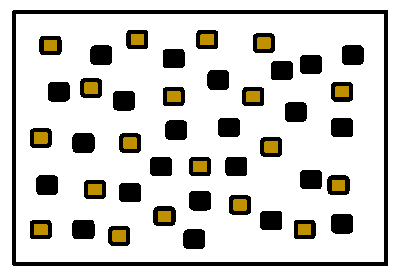
\includegraphics[width=\textwidth]{chapters/chapter4/figures/uniformenv.pdf}
                \caption{Uniform}
                \label{fig:uniformenv}
        \end{subfigure}%
        \begin{subfigure}[b]{0.205\textwidth}
                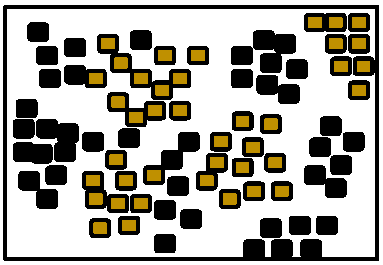
\includegraphics[width=\textwidth]{chapters/chapter4/figures/clusterenv.pdf}
                \caption{Clustered}
                \label{fig:clusterenv}
        \end{subfigure}
        \begin{subfigure}[b]{0.2\textwidth}
                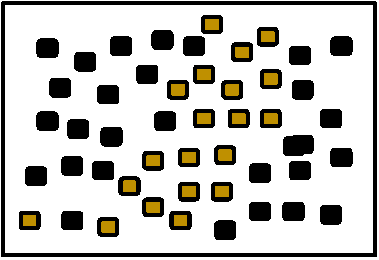
\includegraphics[width=\textwidth]{chapters/chapter4/figures/veinenv.pdf}
                \caption{Vein}
                \label{fig:veinenv}
        \end{subfigure}  
        \begin{subfigure}[b]{0.2\textwidth}
                        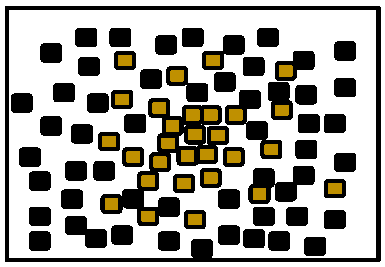
\includegraphics[width=\textwidth]{chapters/chapter4/figures/gaussianenv}
                        \caption{Gaussian}
                        \label{fig:gaussianenv}
       \end{subfigure}
        \caption{Environment Classes}\label{fig:environments}
\end{figure}


%%%%%%%%%%%%%%%%%%%%%%%%%%%%%%%%%%%%%%%%%%%%%%%%%
%%%%%%%%%%%%%%%%%%%%%%%%%%%%%%%%%%%%%%%%%%%%%%%%%
\section{Summary}
\label{third:summary}

This section details the parameters chosen for the algorithms as well as the performance measures selected in order to compare various aspects of the algorithms: the different percentages of each type of item foraged as well as the time spent waiting by the sink. Lastly, the environment types that were generated for experimentation in order to test different properties of the algorithms are discussed. The environment types defined have the four following distributions: uniform distribution, Gaussian distribution, clustered distribution and vein distribution. 


%%%
%%%%%%%%%%%%%%%%%%%%%%%%%%%%%%%%%%%%%%%%%%%%%%%%%
%%%%%%%%%%%%%%%%%%%%%%%%%%%%%%%%%%%%%%%%%%%%%%%%% % rename as required (but remember to update directories appropriately)

%%%%%%%%%%%%%%%%%%%%%%%%%%%%%%%%%%%%%%%%%%%%%%%%%
%%%%%%%%%%%%%%%%%%%%%%%%%%%%%%%%%%%%%%%%%%%%%%%%%
\chapter{Results}
\label{chap:results}
Section \ref{overview} focuses on providing a general overview of algorithm performances, and the motivation for the development of an algorithm that can adapt to item type ratio is presented in section \ref{relationship}. Section \ref{Adaptability} highlights how efficiently the honey bee algorithm adapts to item type ratio. %Analysis of the other performance measures, a discussion of the performance per individual environment type,  as well as scalability study for grid sizes, number of robots and percentage of objects, will be left for a future publication. 

\subsection{General Overview}
\label{overview}
When comparing two foraging algorithms, a pairwise Wilcoxon test was performed to determine if a statistical difference occurs, at a significance level of 95\%. The test was performed over all environments. The null  hypothesis is that the results of the two algorithms come from the same distribution. Table \ref{summarytable} gives a final algorithm ranking where 2 is the best performing algorithm and 0 is the worst performing algorithm.


\vspace{-2em}
\begin{table}
\centering
    \caption{The overall Pairwise Mann Whitney U ranking, averages and standard deviations of for $\sigma$ for each algorithm}
        \label{summarytable}
    \begin{tabular}{l|lll}
    \hline \hline
    Algorithms & Wins & Average & Std Dev \\ \hline
    Naive      & 0    & 0.528   & 0.394  \\
    Desert Ant  & 1    & 0.643   & 0.387  \\
    Honey Bee   & 2    & 0.807   & 0.294  \\

    \hline
    \end{tabular}

\end{table}
Statistical tests indicate a significant difference between the results of all algorithms. Desert ant foraging performed better than na\"ive foraging showing the positive effect of site fidelity. The honey bee algorithm out-performed the na\"ive foraging algorithm and desert ant algorithm indicating the positive effect of communication and adaptivity of the honey bee foraging algorithm. The standard deviation is high for all algorithms due to the extremely large variations in the environments provided.

\subsection{Analysis of Relationship between Item Ratio in Environment and Item Ratio of Robots}
\label{relationship}

The following hypotheses are addressed:
\begin{enumerate}
\item An algorithm that forages a portion of non-prioritized items will have greater performance than an algorithm that does not forage any non-prioritized items.
\item Algorithm performance depends on the $r$ as well as $\tau$ and that as $r$ increases, the value of $\tau$ that yields the greatest value of $\sigma$, $\tau_{best}$, will increase approximately linearly for the na\"ive and desert ant algorithms.
\end{enumerate}

An algorithm configured with $\tau=1$ is where only prioritized items are foraged. Analysing Table \ref{ratio}, for the na\"ive and desert ant algorithms, for all values of $r$ where $r \neq 1$, $\tau_{best}$ is never equal to $1$, proves the hypothesis that the algorithms achieved the best performance when some robots are configured to forage non-prioritized items. The result may be because non-prioritized items are moved out of the way to allow for easier, faster access to prioritized items or allow access to inaccessible prioritized items.


\begin{table} [h]
     \caption{The performance, $\sigma$, for each foraging algorithm, for each combinations of $r$ and $\tau$. If $\tau_{best}$ exists, $\tau_{best}$ is provided. The best value of $\sigma$ is shown in bold.}
     \label{ratio}
	\centering
    \begin{tabular}{|c|c||l|l|l|l|l|l|l|l|l||l|}
	\hline    & & \multicolumn{9}{ |c|| } {$\tau$} &   \\ 
    \cline{3-11}
\multirow{-2}{*}{Algorithm}  &  \multirow{-2}{*}{$r$} & 0     & 0.2   & 0.25  & 0.333 & 0.5   & 0.667  & 0.75  & 0.8    & 1   & \multirow{-2}{*}{$\tau_{best}$ } \\ \hline
    &0     & 1 & 1     & 1     & 1     & 1     & 1     & 1     & 1     & 1     & \\
    &0.2   & 0 & 0.492 & 0.526 & 0.567 & \textbf{0.597} & 0.595 & 0.587 & 0.577 & 0.471 & 0.5 \\
    &0.25  & 0 & 0.484 & 0.526 & 0.557 & 0.588 & \textbf{0.595} & 0.585 & 0.575 & 0.477 & 0.667\\
    &0.333 & 0 & 0.467 & 0.507 & 0.544 & 0.586 & \textbf{0.596} & 0.592 & 0.584 & 0.495 & 0.667\\
    &0.5   & 0 & 0.428 & 0.46  & 0.508 & 0.568 & 0.588 & \textbf{0.591} & 0.589 & 0.528 & 0.75\\
    &0.667 & 0 & 0.4   & 0.433 & 0.487 & 0.544 & 0.583 & \textbf{0.591} & 0.593 & 0.554 & 0.75 \\
    &0.75  & 0 & 0.377 & 0.425 & 0.47  & 0.531 & 0.576 & 0.585 & \textbf{0.591} & 0.567 & 0.8\\
    &0.8   & 0 & 0.372 & 0.409 & 0.455 & 0.53  & 0.571 & 0.584 & \textbf{0.592} & 0.575 & 0.8\\
\multirow{-9}{*}{Na\"ive}&    1     & 0 & 0.336 & 0.375 & 0.433 & 0.5   & 0.552 & 0.57  & 0.581 & \textbf{0.618} & 1\\
     \hline
 &   0                    & 1 & 1     & 1     & 1     & 1     & 1     & 1     & 1     & 1       &    \\
&    0.2                  & 0 & 0.698 & 0.724 & \textbf{0.737} & \textbf{0.737} & 0.712 & 0.694 & 0.67  & 0.519 & 0.333\\
&    0.25                 & 0 & 0.678 & 0.711 & 0.73  & \textbf{0.735} & 0.715 & 0.697 & 0.673 & 0.530 & 0.5 \\
&    0.333                & 0 & 0.65  & 0.693 & 0.722 & \textbf{0.739} & 0.725 & 0.71  & 0.686 & 0.562 & 0.5\\
&    0.5                  & 0 & 0.596 & 0.645 & 0.684 & 0.729 & \textbf{0.734} & 0.725 & 0.701 & 0.621 & 0.667\\
&    0.667                & 0 & 0.554 & 0.607 & 0.648 & 0.706 & 0.737 & \textbf{0.738} & 0.716 & 0.675 & 0.75\\
&    0.75                 & 0 & 0.533 & 0.587 & 0.63  & 0.691 & 0.731 & \textbf{0.739} & 0.72  & 0.703  & 0.75 \\
&    0.8                  & 0 & 0.523 & 0.577 & 0.62  & 0.682 & 0.725 & 0.736 & \textbf{0.74}  & 0.718 & 0.8\\
\multirow{-9}{*}{Desert Ant}&    1                    & 0 & 0.488 & 0.543 & 0.588 & 0.654 & 0.702 & 0.718 & 0.726 & \textbf{0.758} & 1\\ \hline
    %Honey Bee
&        0  & 1     & 1     & 1     & 1     & 1     & 1     & 1     & 1     & 1  &   \\
&    0.2                  & \textbf{0.687} &\textbf{0.687} & 0.686 & 0.686 & 0.686 & 0.685 & 0.686 & 0.685 & \textbf{0.687} &\\
&    0.25                 & 0.678 & \textbf{0.679} & 0.678 & 0.678 &\textbf{0.679} & \textbf{0.679} & 0.678 & 0.677 & \textbf{0.679} &\\
&    0.333                & \textbf{0.674} & \textbf{0.674} & \textbf{0.674} & \textbf{0.674} & \textbf{0.674} & \textbf{0.674} & 0.673 & \textbf{0.674} &\textbf{0.674} &\\
&    0.5                  & 0.668 & \textbf{0.669} & 0.668 & 0.668 & 0.668 & 0.668 & 0.668 & 0.668 & \textbf{0.669} &\\
&    0.667                & 0.671 & 0.671 & 0.671 & 0.671 & 0.671 & \textbf{0.672} & 0.671 & 0.671 & 0.671 &\\
&    0.75                 & 0.672 & \textbf{0.673} & 0.671 & 0.671 & 0.672 &\textbf{0.673} & 0.672 & \textbf{0.673} & \textbf{0.673}&\\
&    0.8                  & 0.674 & 0.674 & 0.674 & 0.674 & 0.674 & \textbf{0.675} &  \textbf{0.675} &  \textbf{0.675} & \textbf{0.675}& \\
\multirow{-9}{*}{Honey Bee}&    1                    & \textbf{0.691} & 0.69  & \textbf{0.691} & 0.69  & \textbf{0.691} &  \textbf{0.691}& 0.69  & 0.69  & 0.69  &\\ \hline

    \end{tabular}

\end{table}

Fig \ref{desertantplot} shows the region in parameter space where the desert ant algorithm performs the best. The na\"ive and desert ant algorithms performed best when $\tau$ was slightly greater than $r$. The existence of the relationship motivates the development of an algorithm that adapts $\tau$ to correspond the environment item ratio $r$.

\begin{figure}[!htb]
\centering
\resizebox{0.8\textwidth}{!}{% GNUPLOT: LaTeX picture with Postscript
\begingroup
  \makeatletter
  \providecommand\color[2][]{%
    \GenericError{(gnuplot) \space\space\space\@spaces}{%
      Package color not loaded in conjunction with
      terminal option `colourtext'%
    }{See the gnuplot documentation for explanation.%
    }{Either use 'blacktext' in gnuplot or load the package
      color.sty in LaTeX.}%
    \renewcommand\color[2][]{}%
  }%
  \providecommand\includegraphics[2][]{%
    \GenericError{(gnuplot) \space\space\space\@spaces}{%
      Package graphicx or graphics not loaded%
    }{See the gnuplot documentation for explanation.%
    }{The gnuplot epslatex terminal needs graphicx.sty or graphics.sty.}%
    \renewcommand\includegraphics[2][]{}%
  }%
  \providecommand\rotatebox[2]{#2}%
  \@ifundefined{ifGPcolor}{%
    \newif\ifGPcolor
    \GPcolorfalse
  }{}%
  \@ifundefined{ifGPblacktext}{%
    \newif\ifGPblacktext
    \GPblacktexttrue
  }{}%
  % define a \g@addto@macro without @ in the name:
  \let\gplgaddtomacro\g@addto@macro
  % define empty templates for all commands taking text:
  \gdef\gplbacktext{}%
  \gdef\gplfronttext{}%
  \makeatother
  \ifGPblacktext
    % no textcolor at all
    \def\colorrgb#1{}%
    \def\colorgray#1{}%
  \else
    % gray or color?
    \ifGPcolor
      \def\colorrgb#1{\color[rgb]{#1}}%
      \def\colorgray#1{\color[gray]{#1}}%
      \expandafter\def\csname LTw\endcsname{\color{white}}%
      \expandafter\def\csname LTb\endcsname{\color{black}}%
      \expandafter\def\csname LTa\endcsname{\color{black}}%
      \expandafter\def\csname LT0\endcsname{\color[rgb]{1,0,0}}%
      \expandafter\def\csname LT1\endcsname{\color[rgb]{0,1,0}}%
      \expandafter\def\csname LT2\endcsname{\color[rgb]{0,0,1}}%
      \expandafter\def\csname LT3\endcsname{\color[rgb]{1,0,1}}%
      \expandafter\def\csname LT4\endcsname{\color[rgb]{0,1,1}}%
      \expandafter\def\csname LT5\endcsname{\color[rgb]{1,1,0}}%
      \expandafter\def\csname LT6\endcsname{\color[rgb]{0,0,0}}%
      \expandafter\def\csname LT7\endcsname{\color[rgb]{1,0.3,0}}%
      \expandafter\def\csname LT8\endcsname{\color[rgb]{0.5,0.5,0.5}}%
    \else
      % gray
      \def\colorrgb#1{\color{black}}%
      \def\colorgray#1{\color[gray]{#1}}%
      \expandafter\def\csname LTw\endcsname{\color{white}}%
      \expandafter\def\csname LTb\endcsname{\color{black}}%
      \expandafter\def\csname LTa\endcsname{\color{black}}%
      \expandafter\def\csname LT0\endcsname{\color{black}}%
      \expandafter\def\csname LT1\endcsname{\color{black}}%
      \expandafter\def\csname LT2\endcsname{\color{black}}%
      \expandafter\def\csname LT3\endcsname{\color{black}}%
      \expandafter\def\csname LT4\endcsname{\color{black}}%
      \expandafter\def\csname LT5\endcsname{\color{black}}%
      \expandafter\def\csname LT6\endcsname{\color{black}}%
      \expandafter\def\csname LT7\endcsname{\color{black}}%
      \expandafter\def\csname LT8\endcsname{\color{black}}%
    \fi
  \fi
  \setlength{\unitlength}{0.0500bp}%
  \begin{picture}(7200.00,5040.00)%
    \gplgaddtomacro\gplbacktext{%
      \csname LTb\endcsname%
      \put(946,704){\makebox(0,0)[r]{\strut{} 0.2}}%
      \put(946,1213){\makebox(0,0)[r]{\strut{} 0.3}}%
      \put(946,1722){\makebox(0,0)[r]{\strut{} 0.4}}%
      \put(946,2231){\makebox(0,0)[r]{\strut{} 0.5}}%
      \put(946,2740){\makebox(0,0)[r]{\strut{} 0.6}}%
      \put(946,3248){\makebox(0,0)[r]{\strut{} 0.7}}%
      \put(946,3757){\makebox(0,0)[r]{\strut{} 0.8}}%
      \put(946,4266){\makebox(0,0)[r]{\strut{} 0.9}}%
      \put(946,4775){\makebox(0,0)[r]{\strut{} 1}}%
      \put(1078,484){\makebox(0,0){\strut{} 0.2}}%
      \put(1794,484){\makebox(0,0){\strut{} 0.3}}%
      \put(2509,484){\makebox(0,0){\strut{} 0.4}}%
      \put(3225,484){\makebox(0,0){\strut{} 0.5}}%
      \put(3940,484){\makebox(0,0){\strut{} 0.6}}%
      \put(4656,484){\makebox(0,0){\strut{} 0.7}}%
      \put(5372,484){\makebox(0,0){\strut{} 0.8}}%
      \put(6087,484){\makebox(0,0){\strut{} 0.9}}%
      \put(6803,484){\makebox(0,0){\strut{} 1}}%
      \put(176,2739){\rotatebox{-270}{\makebox(0,0){\strut{}$\tau$}}}%
      \put(3940,154){\makebox(0,0){\strut{}$r$}}%
    }%
    \gplgaddtomacro\gplfronttext{%
      \csname LTa\endcsname%
      \put(5381,3757){\makebox(0,0)[l]{\strut{}  0.74}}%
      \csname LT0\endcsname%
      \put(5372,4688){\makebox(0,0)[l]{\strut{} 0.72}}%
      \put(6209,3503){\makebox(0,0)[l]{\strut{}  0.72}}%
      \put(1187,958){\makebox(0,0)[l]{\strut{} 0.72}}%
      \csname LT1\endcsname%
      \put(4418,4154){\makebox(0,0)[l]{\strut{} 0.7}}%
      \put(5372,2587){\makebox(0,0)[l]{\strut{}  0.7}}%
      \csname LT2\endcsname%
      \put(4418,4655){\makebox(0,0)[l]{\strut{} 0.68}}%
      \put(5469,2231){\makebox(0,0)[l]{\strut{}  0.68}}%
      \csname LT3\endcsname%
      \put(3225,4277){\makebox(0,0)[l]{\strut{}  0.66}}%
      \put(6201,2307){\makebox(0,0)[l]{\strut{}  0.66}}%
      \csname LT4\endcsname%
      \put(3225,4530){\makebox(0,0)[l]{\strut{}  0.64}}%
      \put(5372,1654){\makebox(0,0)[l]{\strut{}  0.64}}%
      \csname LT5\endcsname%
      \put(2032,4299){\makebox(0,0)[l]{\strut{}  0.62}}%
      \put(5386,1382){\makebox(0,0)[l]{\strut{}  0.62}}%
      \csname LT6\endcsname%
      \put(2032,4462){\makebox(0,0)[l]{\strut{}  0.6}}%
      \put(6267,1382){\makebox(0,0)[l]{\strut{}  0.6}}%
      \csname LT7\endcsname%
      \put(2032,4625){\makebox(0,0)[l]{\strut{}  0.58}}%
      \put(5372,986){\makebox(0,0)[l]{\strut{}   0.58}}%
      \csname LT8\endcsname%
      \put(1436,4564){\makebox(0,0)[l]{\strut{}  0.56}}%
      \put(6087,958){\makebox(0,0)[l]{\strut{}   0.56}}%
      \csname LT0\endcsname%
      \put(1436,4706){\makebox(0,0)[l]{\strut{}  0.54}}%
    }%
    \gplbacktext
    \put(0,0){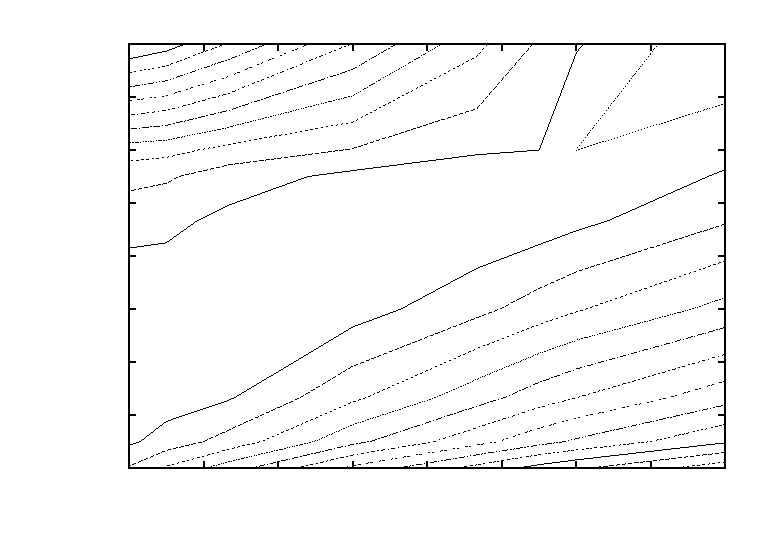
\includegraphics{chapters/chapter6/desertantplot}}%
    \gplfronttext
  \end{picture}%
\endgroup
}
\caption{Contour plot of values for $\sigma$ over values for $r$ and $\tau$ for desert ant foraging}
\label{desertantplot}
\end{figure}

 %But why? Give reason 
%The nai\"ve foraging algorithm slowly clear an entire area around the sink. If there is an equal ratio of robot types to item types then this area would be cleared effectively. 
 %fact that in the more organized environments such as gaussian or vein, it is 

\subsection{Adaptability of the Honey Bee Foraging Algorithm to Item Type Ratio and Comparison to the Na\"ive the Desert Ant Algorithms for Na\"ive and Desert Ant Algorithms}
\label{Adaptability}
Analysis of Table \ref{ratio} indicates that the honey bee foraging algorithm has similar performance throughout all configurations for $r$ and $\tau$, which highlights that the performance of the honey bee algorithm is independent of the configuration of $\tau$, resulting in an algorithm that is more flexible and robust. This could mean that the honey bee algorithm could perform well in dynamic environments where robots and items can be destroyed.

However, according to Table \ref{ratio}, the desert ant algorithm performs better than the honey bee algorithm, for particular configurations of $r$ and $\tau$. This indicates that, if the value of $r$ is known for a particular environment, then it is beneficial to use desert ant foraging and choose $\tau$ appropriately. A possible reason why the desert ant algorithm performs better when optimally configured for a particular environment than the honey bee algorithm is that the honey bee algorithm takes time to adapt to the environment, while the desert ant algorithm with optimal configurations has no division of labour overhead and may outperform the honey bee algorithm under those circumstances.


%\begin{figure}
%\input{naiveplot.tex}
%\caption{Contour plot of values for $\sigma$ over values for $r$ and $\tau$ for nai%\"ve foraging}
%\end{figure}


%\subsection{Energy}

%Due to the waiting state, the honey bee algorithm should  saving energy and thus be more energy efficient. The amount of time spent in a waiting state was measured, however surprisingly, not much time was spent waiting overall. This indicates that there is room for improvement from an energy perspective.

%%%%%%%%%%%%%%%%%%%%%%%%%%%%%%%%%%%%%%%%%%%%%%%%%
\section{Summary}
\label{results:summary}

%%%%%%%%%%%%%%%%%%%%%%%%%%%%%%%%%%%%%%%%%%%%%%%%%
%%%%%%%%%%%%%%%%%%%%%%%%%%%%%%%%%%%%%%%%%%%%%%%%% % rename as required (but remember to update directories appropriately)
% add all other chapters you decide to write (also create an appropriate directory structure)
%%%%%%%%%%%%%%%%%%%%%%%%%%%%%%%%%%%%%%%%%%%%%%%%%
%%%%%%%%%%%%%%%%%%%%%%%%%%%%%%%%%%%%%%%%%%%%%%%%%

\chapter{Conclusions}
\label{chap:conclusions}

This chapter provides an overview of the conclusions arrived at in this work. For ease of reference, the research objectives which were given at the outset of this thesis are reiterated in Section~\ref{sec:introduction:objectives}, while Section~\ref{sec:introduction:contributions} summarizes the novel contributions made by the research. A synopsis of the experimental findings of this thesis are presented in Section~\ref{sec:conclusions:conclusion_summary}, while possible future work is  summarises the conclusions derived at by the research performed, while Section~\ref{sec:conclusions:sec:conclusions:future_work} outlines possible future work that can be performed.


\section{Objectives}
\label{sec:introduction:objectives}

The primary objectives of this thesis are as follows: To

\begin{itemize}
	\item conduct a survey of the swarm robotics field;
	\item conduct a survey of foraging in social insects and  swarm robotics;
	\item define the prioritized foraging problem;
	\item propose metrics for evaluating the performance of swarm robotics algorithms on the prioritized foraging problem;
	\item propose and develop different nature-inspired algorithms in a simulated swarm robotic environment, to be evaluated on the prioritized foraging problem; and
	\item evaluate the efficiency, flexibility, scalability, and robustness of the nature-inspired algorithms over different environments and different swarm configurations, on the prioritized foraging problem.
\end{itemize}

%%%%%%%%%%%%%%%%%%%%%%%%%%%%%%%%%%%%%%%%%%%%%%%%%
%%%%%%%%%%%%%%%%%%%%%%%%%%%%%%%%%%%%%%%%%%%%%%%%%


\section{Summary of Conclusions}
\label{sec:conclusions:conclusion_summary}

The first contribution of this research was to introduce a novel variation of the swarm robotics multiforaging problem, denoted the prioritized foraging problem. The prioritized foraging problem differs from other multi-foraging swarm robotics problems in that the two types of items that need to be foraged have different priorities. One type of item has a high priority to be foraged, while the other type of item has a lower priority of being foraged. The prioritized foraging problem is a novel way of modelling the real-world problem of search and rescue.  

This research then reviewed and selected appropriate existing swarm robotics foraging algorithms to be evaluated on the prioritized foraging problem. A novel honeybee inspired foraging algorithm is also developed. The division of labour between of honeybees between different types of food during times of stressed was specifically modelled in the honeybee inspired algorithm.

In order to evaluate the selected algorithms on the prioritized foraging problem, methods for generating prioritized foraging environments, with different environment item type ratios and with clustered, uniform, gaussian, and vein distributions of items, was presented. Performance measures were defined to evaluate each algorithm on the prioritized foraging problem, in terms of their efficiency, scalability, flexibility, and robustness. 

Results showed that the honey bee algorithm was the most efficient over all environments and swarm configurations, while the desert ant was the next most efficient and the na\"ive algorithm was the least efficient.

Flexibility was analysed in terms of flexibility over different environments prioritized item ratio and flexibility over different environment distribution types. The honey bee algorithm was determined to be the most flexible in terms of an environments prioritized item ratio, which was demonstrated to be a result of its ability to adapt the swarm's specialization ratio to more suitably forage a given environment. The na\"ive algorithm was more flexible than the desert ant algorithm in terms of environment item distribution. The na\"ive algorithm's flexibility is attributed to the fact that the na\"ive algorithm is less efficient across all environment item ratios. This suggests that the na\"ive algorithm appears flexible only because it performs equally bad across all environment item distributions.

The honey bee algorithm is the most flexible over different types of environmental distributions, followed by the desert ant algorithm, and lastly the na\"ve algorithm. The honey bee algorithm was determined to be more flexible, due to it's ability to adapt the specialization ratio to better suit the environment ratio of the accessible environment. The adaptation of specialization ratio allowed the honey bee swarm to focus on foraging non-prioritized items when only non-prioritized items were accessible, and then adjust the ratio to focus on foraging prioritized items when more prioritized items became accessible. The desert ant and na\"ive algorithms were shown to be less flexible than the honey bee algorithm. 

The scalability in terms of swarm scalability, was determined to be sub-linear. The na\"ive algorithm was the most scalable in terms of swarm density, followed by the desert ant algorithm and honey bee algorithm which exhibited similar scalability. The desert ant algorithm's poor performance, compared to the na\"ive algorithm, was attributed the desert ant algorithm's use of site fidelity. The desert ant algorithm's site fidelity increased inter-robot interference, which resulted in decreased efficiency when swarm density was high. The honey bee algorithm was shown to be slightly more scalable than the desert ant algorithm, due to the honey bee algorithm's attempt to regulate the number of active foragers by division of labour. The difference in swarm scalability between the desert ant algorithm and the honey bee algorithm was very small, suggesting that the regulation of active foragers was not functioning very well. The honey bee algorithm's ability to regulate the number of active foragers as swarm density increases was shown to be ineffective. 

The honey bee algorithm was the most scalable in terms of the problem density , followed by the na\"ive algorithm, and lastly the desert ant algorithm. Discussion revealed that the desert ant algorithm performed comparatively worse than the na\"ive algorithm in terms of problem scalability, due to the desert ant algorithm's use of site fidelity to exploit good search areas. The section determined the na\"ive algorithm's ability to explore more than the desert ant algorithm resulted in better problem scalability. The honey bee algorithm was the most scalable in terms of problem scalability. The problem scalability of the honey bee algorithm can be attributed to the ability of the honey bee algorithm to adapt $\tau$ to help clear non-prioritized items, which resulted in lower inter-robot and environmental interference, which in turn increased the foraging efficiency.

Robustness of the algorithms was evaluated in terms of redundancy and decentralized coordination. Evidence showed that the honey bee algorithm was the most redundant, because the swarm is completely homogeneous. The division of labour mechanisms of the honey bee swarm allow each robot to switch their item specialization. The desert ant algorithm and na\"ive algorithm robots can only forage a single item type, which is pre-configured, and thus their swarms are heterogeneous, resulting in lower redundancy.

The coordination between robots of the desert ant and na\"ive algorithms was determined to be more decentralized than the coordination of robots in the honey bee algorithm. The honey bee algorithm's coordination mechanisms were shown to be sensitive to faults in specific swarm individuals where invalid information was communicated to the swarm, and the communication of invalid information impacted the overall swarm efficiency. 


%%%%%%%%%%%%%%%%%%%%%%%%%%%%%%%%%%%%%%%%%%%%%%%%%
%%%%%%%%%%%%%%%%%%%%%%%%%%%%%%%%%%%%%%%%%%%%%%%%%

\section{Future Work}
\label{sec:conclusions:future_work}

%Enumerate the future work that you could foresee developing from the work you have done here. Mention areas you could not focus on, or possible extensions to your work. It is a good idea to be thorough, since you increase your chances of being referenced by other researchers who follow up on your work, even if you do not do so yourself. You may consider writing this as a bulleted list, if you mention many aspects.

%%%%%%%%%%%%%%%%%%%%%%%%%%%%%%%%%%%%%%%%%%%%%%%%%
%%%%%%%%%%%%%%%%%%%%%%%%%%%%%%%%%%%%%%%%%%%%%%%%%

%%%%%%%%%%%%%%%%%%%%%%%%%%%%%%%%%%%%%%%%%%%%%%%%%
%%%%%%%%%%%%%%%%%%%%%%%%%%%%%%%%%%%%%%%%%%%%%%%%%

\cleardoublepage
\ifpdf
\phantomsection
\fi
\label{bibliography}
\printbibliography

%%%%%%%%%%%%%%%%%%%%%%%%%%%%%%%%%%%%%%%%%%%%%%%%%
%%%%%%%%%%%%%%%%%%%%%%%%%%%%%%%%%%%%%%%%%%%%%%%%%

\appendix
%%%%%%%%%%%%%%%%%%%%%%%%%%%%%%%%%%%%%%%%%%%%%%%%%
%%%%%%%%%%%%%%%%%%%%%%%%%%%%%%%%%%%%%%%%%%%%%%%%%

\renewcommand{\glossarypreamble}{Provide a short introduction to the appendix here. Mention that acronyms are listed alphabetically and typeset in bold, with the meaning of the acronym alongside. Also note that you must include acronyms using \texttt{useacronym} for them to show up here. If there are no acronyms defined in your text, this introduction will also not be displayed:}

\cleardoublepage
\ifpdf
\phantomsection
\fi
\chapter{Acronyms}
\label{app:acronyms}
\printglossary

%%%%%%%%%%%%%%%%%%%%%%%%%%%%%%%%%%%%%%%%%%%%%%%%%
%%%%%%%%%%%%%%%%%%%%%%%%%%%%%%%%%%%%%%%%%%%%%%%%%
%%%%%%%%%%%%%%%%%%%%%%%%%%%%%%%%%%%%%%%%%%%%%%%%%
%%%%%%%%%%%%%%%%%%%%%%%%%%%%%%%%%%%%%%%%%%%%%%%%%

\chapter{Symbols}
\label{app:symbols}

The following appendix defines the symbols used in each chapter.  


%%%%%%%%%%%%%%%%%%%%%%%%%%%%%%%%%%%%%%%%%%%%%%%%%
%%%%%%%%%%%%%%%%%%%%%%%%%%%%%%%%%%%%%%%%%%%%%%%%%

\section{Chapter~\ref{chap:second}: Foraging}
\label{sec:symbols:foraging}


\begin{description}
	\item[\parbox{\namewidth}{$p1$}] The probability that a robot will changed from rest to searching is adapted upon return to the sink and from deposit to rest.
\end{description}

\section{Chapter~\ref{chap:divisionoflabour}: Division Of Labour}
\label{sec:symbols:divisionoflabour}


\begin{description}
	\item[\parbox{\namewidth}{$R$}] The set of tasks that can be performed by individuals of the swarm.
	\item[\parbox{\namewidth}{$\gamma$}] An individual robot in a swarm.
	\item[\parbox{\namewidth}{$\nu$}] A task such that $\nu \in R$
	\item[\parbox{\namewidth}{$r_{\gamma,\nu}$}] A response threshold for of robot $\gamma$ for task $\nu$.
	\item[\parbox{\namewidth}{$z$}] The probability of a robot to switch from search behaviour to rest behaviour.
\end{description}


%%%%%%%%%%%%%%%%%%%%%%%%%%%%%%%%%%%%%%%%%%%%%%%%%
%%%%%%%%%%%%%%%%%%%%%%%%%%%%%%%%%%%%%%%%%%%%%%%%%

\section{Chapter~\ref{chap:third}: Nature Inspired Algorithms for Prioritized Foraging}
\label{sec:symbols:foraging}

\begin{description}
\setlength{\itemsep}{-1mm}
	\item[\parbox{\namewidth}{$i$}] The current time step in a swarm robot experiment
	
\item[\parbox{\namewidth}{$state$}] The state a particular robot is in.

\item[\parbox{\namewidth}{$role$}] The role of a particular robot in the honey bee algorithm.

	\item[\parbox{\namewidth}{$i_{state}$}] The current time step of being in consecutive state $state$, where $state$ is any valid state for the robot.
	
	\item[\parbox{\namewidth}{$t_{wait}$}] The maximum time a robot can spend consecutively in wait state.
	
	\item[\parbox{\namewidth}{$t_{ls}$}] The maximum time a robot can spend consecutively in the local search state.
	
	\item[\parbox{\namewidth}{$t_{forage}$}] The maximum time a robot can spend consecutively in the forage state.

	\item[\parbox{\namewidth}{$t_{explore}$}] The maximum time a robot can spend consecutively in the explore state


	\item[\parbox{\namewidth}{$t_{dance}$}] The maximum time a robot can spend consecutively in the recruitment state.
	
	
	\item[\parbox{\namewidth}{$\varsigma$}] The type of an item which can either be prioritized or non-prioritized.

	\item[\parbox{\namewidth}{$\mu_\varsigma$}] The evaluation of the quality of a site of type $\varsigma$.
	
	\item[\parbox{\namewidth}{$\Phi$}] site quality threshold determining whether a the scout robot switches into the dance state. 
	
	\item[\parbox{\namewidth}{$v$}] A robot's path integration vector

	\item[\parbox{\namewidth}{$\omega$}] A memorized path integration vector representing the location of a site.
	
	\item[\parbox{\namewidth}{$\vartheta$}] An item found by a robot.
	\item[\parbox{\namewidth}{$\xi$}] The site where an item is found.

	\item[\parbox{\namewidth}{$\varrho$}] A random number selected from a uniform distribution such that $\varrho\in(0,1)$.
	
	\item[\parbox{\namewidth}{$\rho$}] The probability that a scout robot becomes a forager robot.
	
\item[\parbox{\namewidth}{$k_j$}] is the value captured on the $j-$th distance sensor of a robot.

\item[\parbox{\namewidth}{$n$}] The number of distance sensors.

\item[\parbox{\namewidth}{$d$}] The direction a robot must take to get to the sink.

\item[\parbox{\namewidth}{$\alpha$}] The probability of listening to the details communicated by the scout robot.		

\item[\parbox{\namewidth}{$f_{max}$}] The maximum time a robot will forage for prioritized items, without finding any before switching to foraging a non-prioritized type.

\item[\parbox{\namewidth}{$X$}] The percentage of robots initialized as scout robots.
\end{description}

%%%%%%%%%%%%%%%%%%%%%%%%%%%%%%%%%%%%%%%%%%%%%%%%%
%%%%%%%%%%%%%%%%%%%%%%%%%%%%%%%%%%%%%%%%%%%%%%%%%

\section{Chapter~\ref{chap:experiment}: Experimental Setup}
\label{sec:symbols:foraging}


\begin{description}
	\item[\parbox{\namewidth}{$d$}] Desirability of a direction $i$.
	\item[\parbox{\namewidth}{$i$}] A direction a robot can perceive.
	
	\item[\parbox{\namewidth}{$\kappa_i$}] The clarity which indicates the distance of next nearest obstacle.
	 
	\item[\parbox{\namewidth}{$v$}] The depth of view of a robot's perception.

	\item[\parbox{\namewidth}{$\iota_i$}] The directness of a direction $i$, calculated as the angular deviation from the direction of the destination

	\item[\parbox{\namewidth}{$f$}] The	field of view of a robot's perception.
		
	\item[\parbox{\namewidth}{$\lambda$}] A ratio which determines whether clarity, $\kappa_i$ or directness, $\iota_i$ of direction $i$, has more effect on desirability $d$.
	
	\item[\parbox{\namewidth}{$S$}] The	size of the environment grid.

	\item[\parbox{\namewidth}{$p$}] The density of the items on the grid.

	\item[\parbox{\namewidth}{$r$}] The ratio of prioritized to non-prioritized items.

	\item[\parbox{\namewidth}{$\tau$}] The ratio of robots foraging prioritized items to the ratio of robots foraging non-prioritized items.

	\item[\parbox{\namewidth}{$c$}] The density of robots.

	\item[\parbox{\namewidth}{$\sigma$}] The percentage of prioritized items foraged over time.

	\item[\parbox{\namewidth}{$\mu$}] The percentage of non-prioritized items foraged over time.

	\item[\parbox{\namewidth}{$\epsilon$}] The average time spent by agents waiting at the sink.
	
\end{description}

%%%%%%%%%%%%%%%%%%%%%%%%%%%%%%%%%%%%%%%%%%%%%%%%%
%%%%%%%%%%%%%%%%%%%%%%%%%%%%%%%%%%%%%%%%%%%%%%%%%

\chapter{Derived Publications}
\label{app:derived_publications}

The following publication was derived from this thesis:
\begin{itemize}
	\item Jade Abbott, and Andries P. Engelbrecht. Nature-inspired swarm robotics algorithms for prioritized foraging. In \textit{Proceedings of 9th International Conference on Swarm Intelligence}, pages 246--253, 2014
\end{itemize}

%%%%%%%%%%%%%%%%%%%%%%%%%%%%%%%%%%%%%%%%%%%%%%%%%
%%%%%%%%%%%%%%%%%%%%%%%%%%%%%%%%%%%%%%%%%%%%%%%%%

%%%%%%%%%%%%%%%%%%%%%%%%%%%%%%%%%%%%%%%%%%%%%%%%%
%%%%%%%%%%%%%%%%%%%%%%%%%%%%%%%%%%%%%%%%%%%%%%%%%

\cleardoublepage
\ifpdf
\phantomsection
\fi
\label{index}
\addcontentsline{toc}{chapter}{Index}
\printindex

%%%%%%%%%%%%%%%%%%%%%%%%%%%%%%%%%%%%%%%%%%%%%%%%%
%%%%%%%%%%%%%%%%%%%%%%%%%%%%%%%%%%%%%%%%%%%%%%%%%

\end{document}